\documentclass[12pt,oneside,final]{siuethesis}
\usepackage{microtype} % (optional) for more beautiful typesetting
\usepackage{graphicx} 
\usepackage{hyperref} %makes links clickable
\hypersetup{colorlinks,citecolor=black,filecolor=black,linkcolor=blue,urlcolor=black} %good for electronic copy
\hypersetup{colorlinks,citecolor=black,filecolor=black,linkcolor=black,urlcolor=black}%required for paper graduate school copy
%\usepackage[alphabetic]{amsrefs} %required if using amsrefs, comment out if using bibtex
\usepackage{fixltx2e}
\usepackage{amsmath}
\usepackage{epsf}
%\usepackage{float}
\usepackage{caption}
\usepackage{subfig}
%\usepackage{subcaption}
\usepackage{listings}
\usepackage{rotating}
\usepackage{tabularx}
\usepackage{multirow}

%% controls numbering of theorems
%% this can be configured to your advisor's taste
\newtheorem{theorem}{Theorem}[chapter] %theorem number resets each chapter
\newtheorem{conclusion}[theorem]{Conclusion}
\newtheorem{condition}[theorem]{Condition}
%% conjectures, corollary, defn, etc. numbered sequentially from beginning of chapters
\newtheorem{conjecture}[theorem]{Conjecture} 
\newtheorem{corollary}[theorem]{Corollary}
\newtheorem{example}[theorem]{Example} 
\newtheorem{lemma}[theorem]{Lemma}
\newtheorem{proposition}[theorem]{Proposition}
\newtheorem{solution}[theorem]{Solution}
\theoremstyle{definition}
\newtheorem{definition}[theorem]{Definition}


\author{Bryan Orabutt}
\title{Design and Analysis of a Multi-Channel Discriminator Integrated Circuit for Use in Nuclear Physics Experiments}

%%\advisor{John Q.\ Faculty} %% or 
\advisor{Dr.}{George L. Engel}
\secondreader{Dr.}{Bradley Noble} %% or \secondreader{Dr.}{Karl Gauss}
\thirdreader{Dr.}{Timothy York}
%\fourthreader{Karl Gauss, Sr.}
%\fifthreader{Karl Gauss, Sr.}
%\secondadvisor{Karl Gauss} %if you haves two advisors (rare) then use this line also and pass the option `twoadvisors' to the class
%\abstracttext{Chairperson: The Honorable Jill Smith} %optional -- you can use this to override the text on the abstract page; the grad school default is built-in
\submitdate{August, 2018} %date the month/year submitted to grad school, use a comma between
\copyrightyear{2018} %optional, but required if copyrighted

%% all of these are optional; defaults are shown
\major{Electrical Engineering} 
\degree{Master of Science} %can be used to specify M.A., etc.
\highestdegree{Bachelor of Science} %used if the author already has another graduate degree
\department{Electrical and Computer Engineering} 
%\departmentname{Department}
%\refname{REFERENCES} 

%\captionsetup{width=0.7\textwidth}

\begin{document}
\maketitle 

\frontmatter %signals single spacing/roman numeral pagination

\copyrightpage %optional


% ^^^^^^^^^^^^^^^^^^^^^
% ABSTRACT
% ^^^^^^^^^^^^^^^^^^^^^

\begin{abstract}

\par This thesis presents the design and simulation of a multi-channel integrated circuit (IC) that will be used in nuclear physics experiments. The chip is being designed as a companion chip for another IC used in particle identification called PSD8C. The IC described in this thesis is used to create precise timing pulses for starting time-to-voltage converters (TVCs) on the PSD8C. These timing pulses are created using a technique called Constant Fraction Discrimination (CFD). Each of the sixteen channels in the IC contains a Nowlin circuit, leading-edge discriminator, zero-cross discriminator, and a one shot circuit to generate the output. \par The IC will support input pulse amplitudes between 15 mV and 1.5 V (both positive and negative), and input pulse rise times between 3 nsec and 50 nsec. The IC will feature a programmable output pulse width between 50 nsec and 500 nsec. Most importantly the output pulse firing time variation will be independent of the input amplitude, having a time walk of only 500 psec or less (for input pulse rise time constants of 3 nsec). The IC has been named CFD16C and the design presented is using the AMS-AG 0.35 micron NWELL process.
\end{abstract}


% ^^^^^^^^^^^^^^^^^^^^^^^^^^^^^^^^^^^^^^^
% ACKNOWLEDGEMNTS
% ^^^^^^^^^^^^^^^^^^^^^^^^^^^^^^^^^^^^^^^^


\begin{acknowledgements} 

\par I would first like to thank Dr. George Engel for being a continuous source of guidance through all my time working on this project. I would also like to thank Dr. Bradley Noble for encouraging me to investigate challenging problems and for being a source of guidance both in the classroom and out. I would also thank Dr. Timothy York for introducing me to IC design, without him I likely would never have gone to graduate school. I am grateful to  Dr.  Lee  Sobotka  and  Mr.  Jon  Elson,  department  of  chemistry, Washington  University Saint Louis, for their  help  during  the  various  stages  of  this  project. My  special  thanks  to all of the  faculty  and  staff  of  ECE  department  for  their  direct  and indirect support without which I simply could not have progressed with my work. Additionally, Dr. Gary Mayer of the Computer Science department has helped me expand knowledge beyond the skills learned in the classroom, and I am forever thankful. 
\par I owe a debt of gratitude to my fellow graduate students I've been privileged to work with on this project as well. Pohan Wang, Prarthana Jani, Sneha Edula, and Anil Korkmaz, Sri Kandula, and I all worked together to make CFD16C possible and they have helped make this project a pleasure to work on.
\par I would not have gotten this far without my friends Jack White, Jared Charter, Andrew Quirin, Nelly Sanchez, and Shana Mankouski who have offered support during all of my endeavors in graduate school. I am forever grateful to my family for being a constant source of encouragement. My mother Marsha Orabutt, brother Sean Orabutt, and Vicki Kern, have all been there for me and I know I could not have come this far without them.
\par Special thanks to the National Science Foundation (NSF) for funding the work presented in this thesis under NSF Grant\#1625499.

\end{acknowledgements}

\tableofcontents

\cleardoublepage %cause correct numbering of list of figures

\cleardoublepage

\listoffigures %print list of figures page

\cleardoublepage

\listoftables

\mainmatter %signals single spacing/arabic numeral paginations

% ^^^^^^^^^^^^^^^^^^^^^^^^^^^^^^^^^^^^^^^^^^^^^^^^^^^^^^^^^
%  CHAPTER 1
% ^^^^^^^^^^^^^^^^^^^^^^^^^^^^^^^^^^^^^^^^^^^^^^^^^^^^^^^^^

\chapter{INTRODUCTION}  %% chapter titles must be typed in all caps to conform with regulations

This chapter will introduce the reader to the field of radiation monitoring and describe how custom multi-channel integrated circuits are helping to re-shape this field.  The IC described in this thesis, called CFD16C (Constant Fraction Discriminator--16 Channels), is the newest addition to the family of ICs which are being developed by the IC Design Research Laboratory at Southern Illinois University Edwardsville (SIUE) in collaboration with researchers from the Nuclear Reactions Group at Washington University (WUSTL).

\section{Research Background}

The Integrated Circuits Design Research Laboratory at SIUE and the Nuclear Reactions Group at WUSTL have been working (since 2001) on a family of multi-channel custom integrated circuits.  The group became interested in developing a family of microchips for use in the detection and measurement of ionizing radiation because: (1) the need for high-density signal processing in the low- and intermediate-energy nuclear physics community is widespread, and (2) no commercial chips were identified that were capable of doing what the researchers wanted, and (3) the scientists deemed it necessary for the experimenter to be in the designer's seat. The goal is to develop a ‘‘tool box’’ of circuits,
useful for researchers working with radioactive ion beams, which can be composed in different ways to meet the researchers' evolving needs and desires.

 
The group's first success was an analog shape and peak sensing chip with on-board constant-fraction discriminators and
sparsified readout. This chip is designed for use with arrays of Si strip detectors of medium scale (with the number of channels ranging from a few hundred to a few thousand) and is known as Heavy-Ion Nuclear Physics--16 Channel (HINP16C). 

The second chip, christened Pulse Shape Discrimination--8 Channel(PSD8C), was designed to logically complement (in terms of detector types) the HINP16C chip. PSD8C performs pulse shape discrimination (PSD), and thus particle identification, if the time dependence of the light output of the scintillator depends on particle type. Moreover, PSD8C uses almost all the same supporting hardware as the HINP16C chip. Both ICs were fabricated in the ON-Semiconductor (formerly AMI) 0.5 mm n-well process (C5N), available through MOSIS (see \url{www.mosis.com}).

\begin{figure}[htbp!]
	\centering
 	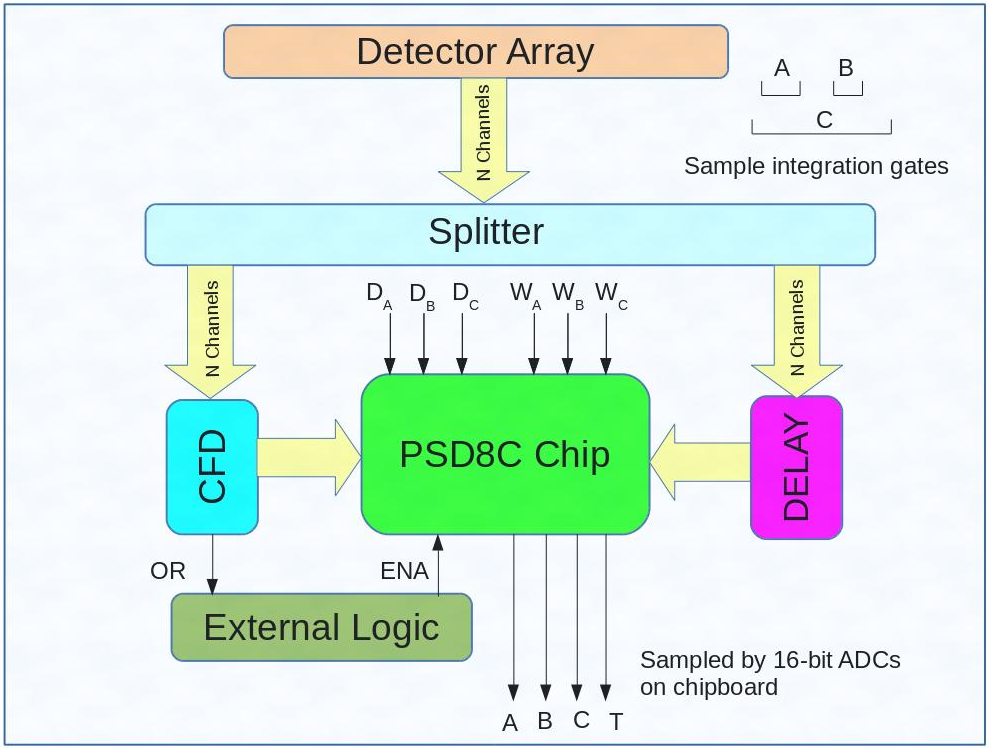
\includegraphics[scale=0.6,keepaspectratio=true]{./ch1_figures/PSD_block.png}
 	\caption{Block diagram of typical PSD system.}
 	\label{FIG:PSD_BLOCK}
\end{figure}

\par Figure~\ref{FIG:PSD_BLOCK} shows a typcial PSD system using the PSD8C IC. The outputs of a detector array are split in two so that a copy of each signal can be sent to both the CFD circuit and the PSD8C. The signals sent to the PSD8C must be delayed to match the propagation delay of the CFD circuit. The CFD logic signals are ANDed with a global enable signal to provide channel enables for the PSD8C. For each delayed detector signal (and it's assosciated CFD logic signal), three integrations (called A, B, C) will be performed with start times referenced to the CFD signals. An additional amplitude, \emph{T}, is produced which is proportional to the time difference between the CFD firing and an external common stop reference, which eliminated the need for VME TDCs.
\par The integrators' starting time delay (D$_{A}$, D$_{B}$, D$_{C}$) and the integration window widths (W$_{A}$, W$_{B}$, W$_{C}$) are controlled by the user. In Figure~\ref{FIG:PSD_BLOCK}, D$_{A}$, D$_{B}$, D$_{C}$ are voltages that are converted to times on-chip, along with the widths W$_{A}$, W$_{B}$, W$_{C}$.

\section{PSD8C IC}

Our PSD8C chip greatly simplifies the pulse-processing electronics needed for large arrays of scintillation detectors. Each channel(see Figure~\ref{FIG:PSD_CHANNEL}) possesses 3 sub-channels. The sub-channels are referred to as A, B, and C. A sub-channel consists of an integrator and a gate generator. External control voltages (DX, WX) determine the gate delay and the gate width. The structure of a single PSD8C sub-channel is illustrated in Figure~\ref{FIG:PSD_SUB_CHANNEL}. Because PSD8C employs (user-controlled) multi-region charge integration, particle identification is incorporated into the basic design. Each channel on the chip also contains a TVC that provides relative time information. The pulse height integrals and the relative time are all stored on capacitors and are either reset, after a user-controlled time, or sequentially read out if acquisition of the event is desired (in a manner similar to that of HINP16C). 

\begin{figure}[htbp!]
	\centering
 	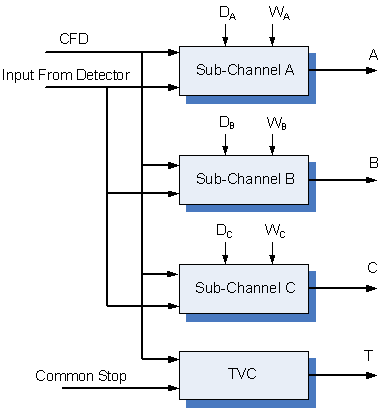
\includegraphics[scale=1.0,keepaspectratio=true]{./ch1_figures/PSD_channel.png}
 	\caption{PSD Channel}
 	\label{FIG:PSD_CHANNEL}
\end{figure}


\begin{figure}[htbp!]
	\centering
 	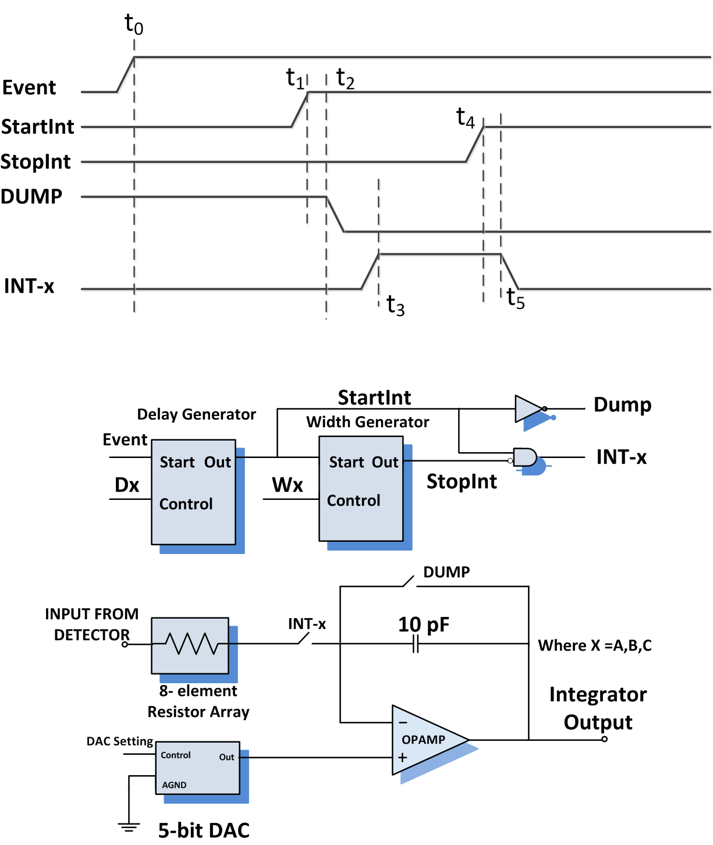
\includegraphics[scale=1.3,keepaspectratio=true]{./ch1_figures/PSD_sub_channel.png}
 	\caption{PSD Sub-channel.}
 	\label{FIG:PSD_SUB_CHANNEL}
\end{figure}

Features of the first generation PSD8C (Rev. 1) chip include:
\begin{itemize}
\item
eight independent channels per IC;
\item
on-chip data sparsification;
\item
each channel automatically resets itself after a user programmable delay time;
\item
three (3) integration regions each with: (a) independent
control of time offset (beginning), (b) width (ending) of the
integration window, and (c) a menu of eight (8) charging rates;
\item
each channel possesses a TVC with two time ranges: 500 ns and 2 ms;
\item
three triggering modes;
\item
fast logical OR-gate and an analog multiplicity output to aid in
trigger decisions;
\item
two power modes to facilitate use with fast and slow detectors
and to thus allow for a more modest power budget for the
latter; 
\item
and CFD circuits are not on-chip so as to provide greater flexibility.
\end{itemize}

PSD8C is described in detail in \cite{PROCTOR} and \cite{HALL}. PSD8C is 2.25 by 5.7 $mm^2$ and is packaged in a 14 by 14 $mm^2$, 128 lead thin quad flat pack. Power consumption is 65 mW (low-bias mode)and 150 mW (high-bias mode).
A second version (Rev. 2) of PSD8C was submitted for fabrication in May 2010. Rev. 2 attempts to correct several minor
problems. First, the TVC circuit could inadvertently be re-started. In Rev. 2, once the rising edge of the "common stop" signal is detected, the TVC cannot re-start until the channel is reset. Second, undesirable temperature dependence (1 $\frac{nsec}{^{\circ}C}$) in the TVC circuit was identified and traced to the local channel buffer. The buffer was redesigned, and the TVC temperature sensitivity has been greatly reduced (5 $\frac{psec}{^{\circ}C}$ in the 500 nsec mode, 40 $\frac{psec}{^{\circ}C}$ in the 2 msec mode). Third, some TVC crosstalk issues were identified and remedied. Fourth, additional shielding was added to the integrator circuits. Finally, at the system level, the chip-boards (printed-circuit boards) were redesigned to include on-board analog to digital converters, or ADCs. (one for each of the chip's analog output pulse trains).

(Still need to talk about enhancements that were made on PSD4)


\section{Need for an Integrated Circuit}

While not including the timing circuits on PSD made it more flexible, those circuits are needed.  Currently, a large complex board with many ICs produce the timing signals required by the PSD chip. This thesis describes the design of multi-channel integrated circuit which can generate the timing signals for a pair of PSD chips.

\begin{figure}[htbp!]
	\centering
 	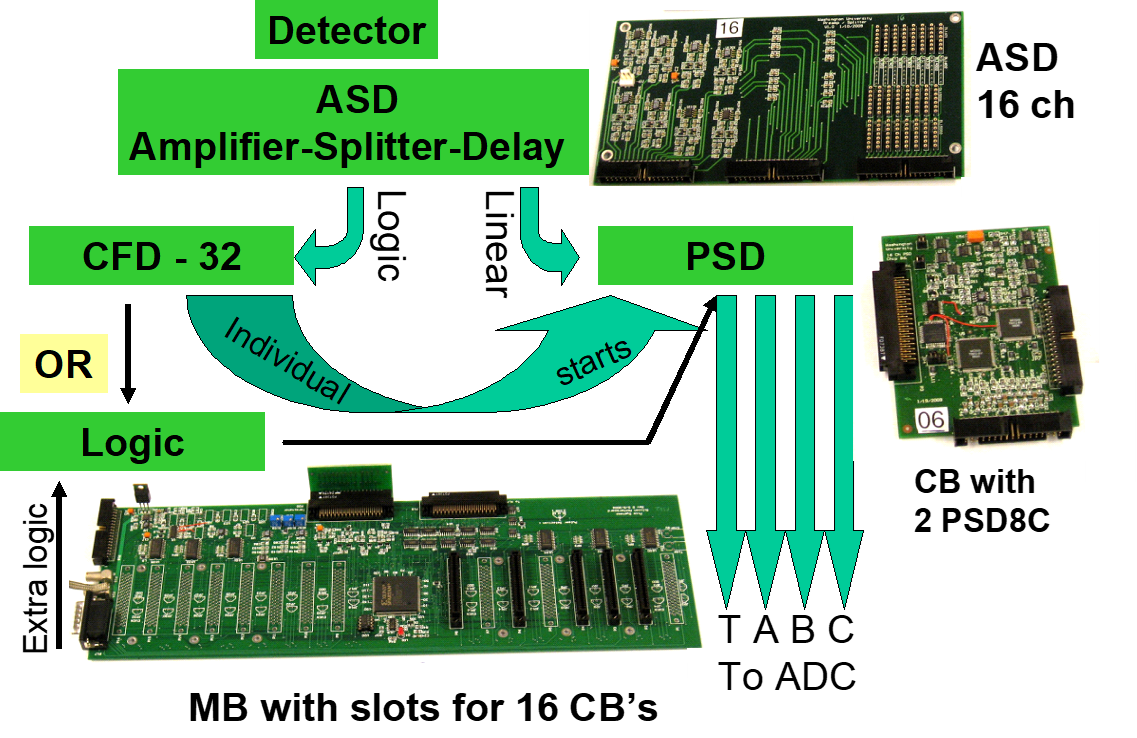
\includegraphics[scale=0.8,keepaspectratio=true]{./ch1_figures/PSD_system.png}
 	\caption{PSD system using board-level CFD electronics}
 	\label{FIG:PSD_SYSTEM}
\end{figure}



\section{Sample Applications}

To focus the reader's attention on what would be possible with the PSD chip complemented by the CFD chip described in this thesis, consider a highly granular discrete element array for neutron detection using the recently developed inorganic \cite{BUDDEN} and plastic \cite{ZAITSEVA} scintillators with PSD. Such a large array would open the n-rich side up to the kind of high-precision work the Washington University group has done on the p-rich side. (The existing work on the neutron-rich side, done at high energy and with detectors such as MONA-LISA \cite{BAUMANNA}, while providing provocative data on such cases as $^{16}\mathrm{Be}$ \cite{SPYROU} and $^{26}\mathrm{O}$ \cite{KOHLEY}, sufferer for poor statistics and, compared to the proton-rich side, poor resolution.) An array to be deployed at low (reaccelerated beam) energies with thousands of optically isolated PSD elements made from the new generation of plastics, would revolutionize the study of multiple n-decay from what are generally high-isospin states. (The problem of detector-to-detector scattering cross-talk can also be improved with discrete pixilation – rather than using large bars – by corrugating the detectors in the same way as the conventional discrete array DEMON has \cite{TILQUIN}).  

While we are enamored with the above idea, it is premature to propose such an array before the ground-work for scalable timing electronics, as we describe in this thesis, is successfully completed. (In fact the coupling of the scintillator – from Eljen – to the new blue sensitive SiPMs – from SensL – is simple compared to the development of the scalable electronics.) To this end however, we plan to develop a circuit board using the PSD and CFD chips to process signals from the new generation of PSD-capable plastic scintillators \cite{ZAITSEVA}. 

The CFD chip described herein with its programmable Nowlin cirucit will allow the WUSTL Nuclear Reactions Group to work with variety of scintillators (LaBr:Ce to CsI:Tl or :Na to standard plastics and, for what might be the most interesting untapped opportunity, the new class of PSD capable plastics \cite{ZAITSEVA}).  


\section{Object and Scope of Work} 

\par The object of this thesis work was to create a multi-channel integrated circuit capable of constant fraction discrimination. This thesis is composed of five chapters. The system level architecture is presented in Chapter 2. Chapter 3 describes the circuit level design of the many sub-circuits that compose the CFD16C. Chapter 4 details the simulated performance of the CFD16C to show that it performs within the intended design specification. Finally Chapter 5 provides a summary, conclusions, and details future work to be done on the CFD16C.

% ^^^^^^^^^^^^^^^^^^^^^^^^^^^^^^^^^^^^^^^^^^^^^^^^^^^^^^^^^
%  CHAPTER 2
% ^^^^^^^^^^^^^^^^^^^^^^^^^^^^^^^^^^^^^^^^^^^^^^^^^^^^^^^^^


\chapter{SYSTEM ARCHITECTURE}

This chapter will attempt to describe the CFD16C integrated circuit at the system-level.  We will start with a detailed list of system requirements and then will describe the high-level architecture of the IC.

\section{System Specifications}
The success of our group over the past 20 years lies on the close working relationship that the IC Design Research Laboratory at Southern Illinois University Edwardsville (SIUE) has had with the Nuclear Reactions Group at Washington University in St. Louis(WUSTL) led by Dr. Lee Sobotka.  The IC group here at SIUE and the Nuclear Reactions Group at WUSTL, after lengthy discussions, drafted the following specifications for the IC described here in this thesis.

\begin{itemize}
\item
The IC should support 16 detectors.
\item
It should support analog pulses of both polarities (relative to analog signal ground).
\item
It should accommodate analog exponentially shaped pulses with rise time constants ranging from 3 nsec to 50 nsec.
\item
It must exhibit "excellent" walk and jitter characteristics for input pulse amplitudes ranging from 15 mV to 1.5 V. The adjective "excellent" will be quantified in a later chapter of this thesis.
\item
Pulse repetition rates up to 1 KHz must be accommodated.
\item
The discriminator in each of the 16 channels should be of the constant fraction type (CFD). In CFD discriminators an attenuated version of the input is subtracted from a delayed version of input waveform and the time at which the difference between the two is equal to zero is used to mark the pulse arrival time. This results in output timing signals independent of pulse amplitude.
\item
Each channel should have a leading-edge threshold.
\item
While the chip must support signals with rise time constants ranging from 3 nsec to 50 nsec, performance will be optimized for the shorter time constants. 
\item
The output pulse width from a channel should be programmable.
\item
The IC should operate from a single 3.3 Volt supply.
\item
Power consumption of the 16 channel IC should not exceed 350 mW \emph{i.e.} 20 mW per channel with 30 mW budgeted for the circuits common to all channels. 
\item
The IC is not to occupy an area greater than roughly 2 mm x 3 mm.  The chip should be packaged in a 64-pin plastic package.  

\end{itemize} 

\section{Features}
\par In order to achieve the intended system design specification many of the analog circuity in the chip is user configurable. Nowlin delay time, leading edge threshold, one-shot pulse width, and lockout times are all able to be configured to the user's needs. Writing to configuration registers is performed using a signal 8-bit wide bus to provide address, mode, and data information. Using the user-controlled \emph{STB} line, address and mode can be presented on the rising edge and then data will be registered into the selected configuration register on the falling edge. Each channel can be individually enabled or disables as per the needs of the user. Additionally, should it be reuqired, all sixteen channels can be disabled with a single global enable pin available to the user. Finally, a test point is provided to give the user feedback about how some of the digital circuit elements within the channel are performing. This test point can come from eight different nodes within a specified signal channel.

\section{System-Level Description}
\par The CFD16C is designed in a 0.35 micron CMOS process. The chip is designed to act as a multi-channel constant fraction discriminator with very low jitter and time walk in the output timing pulse. The chip contains sixteen signal channels that are driven by a detector, and a single common channel that contains circuitry used by all of the signal channels. A system level block diagram of a single signal channel can be seen in Figure~\ref{fig:CFD}.

\begin{figure}[ht]
\centering
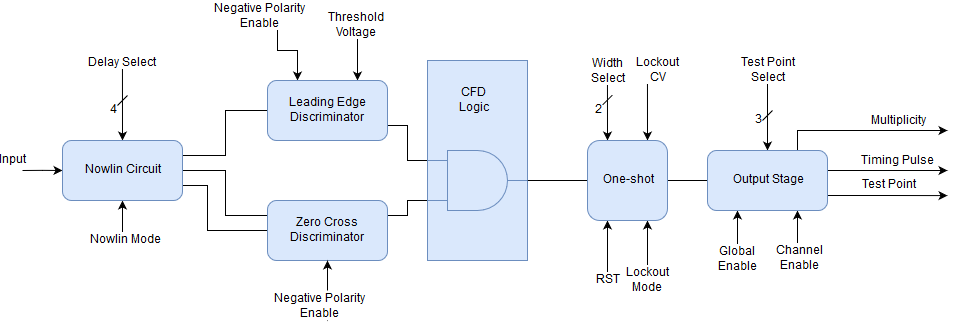
\includegraphics[scale=.47,keepaspectratio=true]{./ch2_figures/channel_block.png} 
\caption{System level overview for one channel of the CFD16C}
\label{fig:CFD}
\end{figure}

\par An analog input pulse will arrive at the input stage of of the channel in the form of an exponential voltage pulse with a rise time $\approx$10 times faster than its fall time. This stage contains a Nowlin circuit that creates a differential output and a high pass filtered output from the input pulse. The differential output is used as input to a zero crossing discriminator while the high pass filtered output is used as input to a leading edge discriminator. The outputs of the two discriminator channels are ANDed together to provide input to a one shot that creates the output timing pulse. Additional outputs such as a test point and multiplicity output are generated in a final output stage of the channel. 

\subsection{Common Channel}
\par The common channel contains configuration registers to change the performance of the various analog circuits in the signal channels. There are a total of three configuration registers in the common channel and one on the signal channel. These registers can be individually selected and loaded by using an special address and mode scheme. Each channel is assigned a 4-bit address from 0000 to 1111 and each register is assigned a 3-bit mode. To load any specific register the correct mode and address must be provided. A fourth bit of mode, the MSB, is used to select all registers of a given mode regardless of what address is provided. Table~\ref{tab:modes} shows the modes and usage for each of the registers.

\begin{figure}[htbp!]
\centering
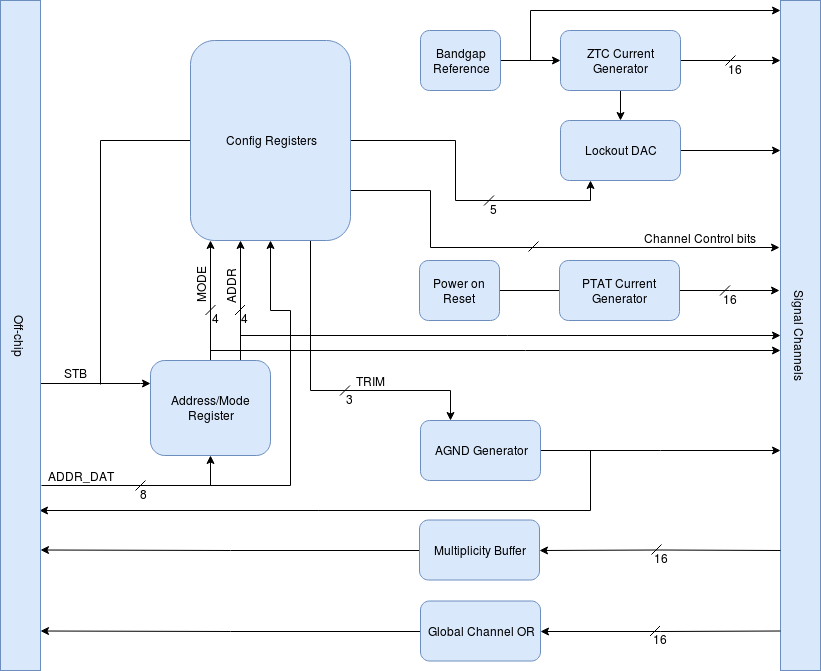
\includegraphics[scale=.5,keepaspectratio=true]{./ch2_figures/common_block.png} 
\caption{System level diagram of the common channel}
\label{fig:common-block}
\end{figure}

\par While the registers need to be provided with data, address, and mode information, only a single 8-bit bus is used to provide this. On the positive edge of the \emph{STB} input address and mode information are stored in a special purpose register that drives the internal \emph{ADDR} and \emph{MODE} busses (see Figure~\ref{fig:addrmode}). On the negative edge of \emph{STB} data is then stored in all enabled registers.
\par The common channel also contains biasing circuitry for many of the analog circuits in the signal channels. Bias currents and reference voltages are generated here and distributed to each of the signal channels. More information on these circuits is presented in Chapter 3.

\begin{figure}[htbp!]
\centering
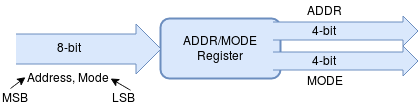
\includegraphics[scale=.7,keepaspectratio=true]{./ch2_figures/data_bus.png} 
\caption{The address, mode, \& data shared bus scheme}
\label{fig:addrmode}
\end{figure}

\subsection{Signal Channel}
\par The input to a signal channel comes from a detector in the form of a pulse with an exponential rise in voltage and an exponential decay. The programmable Nowlin circuit acts as the input stage to the signal channel. The Nowlin circuit is used to create a differential output from this single ended input pulse. One leg of this differential signal is composed of a constant fraction of the input pulse. The other leg of this output is a delayed version of the input pulse. This delay time is determined by an RC time constant that is configurable by changing the value of a programmable capacitor. A high pass filter output is provided by the Nowlin as well, and is used by the leading-edge discriminator circuit.
\par The differential outputs of the Nowlin circuit are used as inputs to a zero-crossing discriminator (Figure~\ref{fig:zcd}). This discriminator is created by cascading several amplifiers together and connecting the final output to a high speed comparator. This circuit will provide a digital output that is a logic high (3.3V) when the two differential output voltages from the Nowlin cross the 0V threshold when referenced to analog ground (\emph{AGND}). This will allow the circuit to produce an output independent of the input pulse amplitude \cite{CFD}. To achieve amplitude independence it is important that the delay time set in the Nowlin circuit is optimal, as seen in Figure~\ref{fig:nowlinout}. With a short delay time there is very little under drive in the output of the final differential amplifier which could prevent the comparator from firing. With too much delay there is not enough slew rate to accommodate the fast timings that are needed.
\par A DC offset cancellation loop is used to remove the effects of systematic DC offsets. Without this DC compensation loop, the output comparator would be permanently stuck in one state regardless of input from the Nowlin circuit. This same DC cancellation loop is also used in the Leading-edge discriminator.

\begin{figure}[htbp!]
\centering
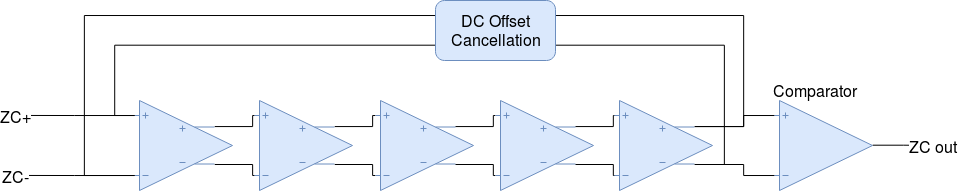
\includegraphics[scale=.45,keepaspectratio=true]{./ch2_figures/zcd.png} 
\caption{Zero cross discriminator with DC cancellation}
\label{fig:zcd}
\end{figure}

\begin{figure}[htbp!]
\centering

\includegraphics[scale=.4,keepaspectratio=true]{./ch2_figures/nowlin.png} 
\caption{Input signal with 3 ns risetime constant showing Nowlin delay effects}
\label{fig:nowlinout}
\end{figure}



\par The input to the leading-edge discriminator comes from the high-pass filter, or "fast shaper", in the Nowlin circuit. The leading-edge discriminator has a user controllable threshold that is compared against the input from the Nowlin circuit. This threshold will be set just above the noise floor, ensuring that the comparator will only fire in response to a real pulse coming off of a detector and not just inherent noise in the circuit. This threshold can be made negative by applying a logic high (3.3V) to the \emph{NEG\_POL} input pin. The output of the leading edge discriminator is then used to qualify the zero-cross detector.

\par Qualified zero-cross discriminator pulse is used as input for a narrow pulse circuit that triggers the one-shot. Figure~\ref{fig:oneshot} shows this in more detail. The oneshot circuit creates the channel's output timing pulse. It is provided with a two bit pulse width seleciton bus that allows the user to configure the output width of this pulse between 50 nsec and 500 nsec. There is another one-shot circuit used to create a lockout period which will prevent the creation of an output timing pulse regardless of the presence of any stimuli from the narrow pulse generator. This lockout time is also user configurable with a control voltage provided by a 5-bit DAC in the common area. The lockout feature can also be completely turned off by the user if desired.

\begin{figure}[h!]
\centering
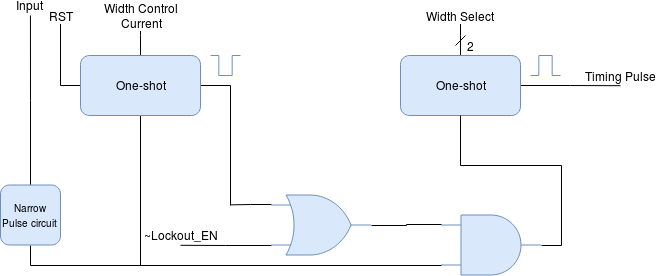
\includegraphics[scale=.65,keepaspectratio=true]{./ch2_figures/oneshot.png} 
\caption{System level diagram of one-shot stage}
\label{fig:oneshot}
\end{figure}

\par A final output generation stage is used to qualify the timing pulse as well and create other useful channel outputs. The timing pulse should not be present on the pin of the chip package if the global enable signal is not present, or the channel enable bit is not set. Therefor the timing pulse is ANDed with these two signals before going off-chip as seen in Figure~\ref{fig:output-qual}. The digital test point, multiplicity, and global channel OR outputs are also created in this stage and explained in more detail in the next chapter.

\begin{figure}[h!]
\centering
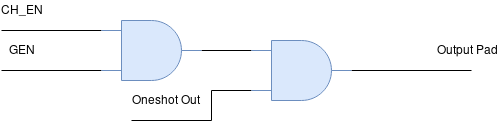
\includegraphics[scale=.7,keepaspectratio=true]{./ch2_figures/output.png} 
\caption{Timing pulse output qualification}
\label{fig:output-qual}
\end{figure}
\section{Chip Pinout}
\par The CFD16C will be packaged in a 64-pin QFN plastic package. The pinout is detailed in Table~\ref{tab:pinout}. Pins with no electrical connection to the chip die are labeled as \emph{NC} (no connection).

\begin{table}[htbp!]
\centering
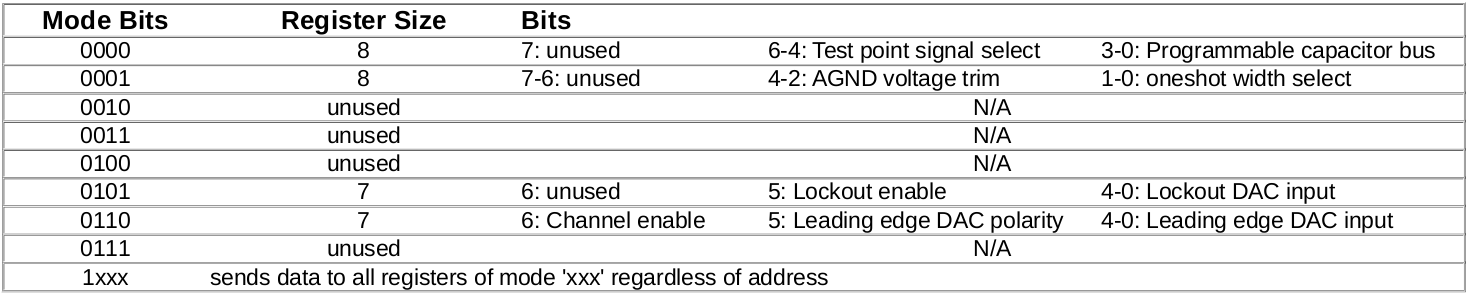
\includegraphics[scale=.35,keepaspectratio=true]{../data/modes.png} 
\caption{Register modes and usage}
\label{tab:modes}
\end{table}

\begin{table}[htbp!]
 \centering
 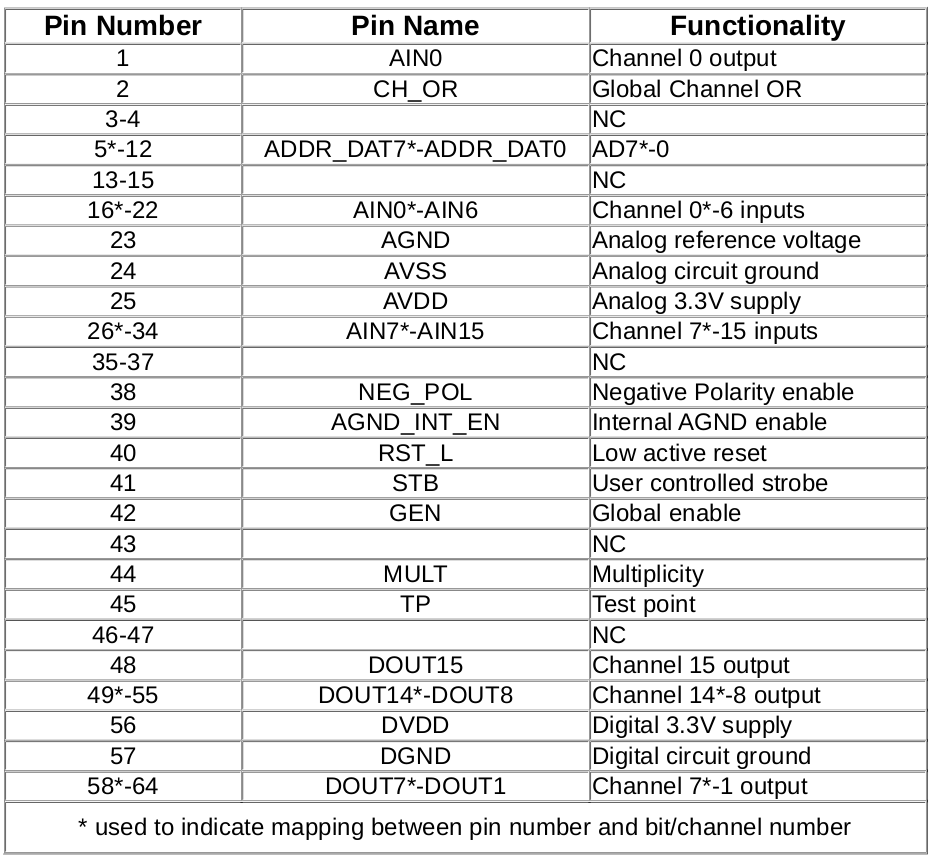
\includegraphics[scale=.35,keepaspectratio=true]{./ch2_figures/pinout.png}
 \caption{Pinout of CFD16C}
 \label{tab:pinout}
\end{table}


% ^^^^^^^^^^^^^^^^^^^^^^^^^^^^^^^^^^^^^^^^^^^^^^^^^^^^^^^^^
%  CHAPTER 3
% ^^^^^^^^^^^^^^^^^^^^^^^^^^^^^^^^^^^^^^^^^^^^^^^^^^^^^^^^^


\chapter{ELECTRICAL LEVEL DESIGN}

\section{Fabrication Process}

The IC described in this thesis will be fabricated in the AMS-AG 0.35 micron NWELL process.  The process supports two poly and 4 metal layers. Double poly capacitors, BJTs, and a high-resistance layer are all available to the designer. NFET device properties are given in Table~\ref{TBL:NMOS_PARMS} while PFET device properties are available in Table~\ref{TBL:PMOS_PARMS}.

% NFET device properties

\begin{table} [htbp!]
\begin{center}
\begin{tabular}{| l | c | c |}
\hline 
Threshold Voltage & $V_{TN}$ & 0.5 V \\ 
\hline 
Transconductance Parameter & $K_{PN}$  &  170 $\frac{\mu A}{V^2}$ \\ 
\hline 
Bulk Modulation Factor & $\gamma_{N}$  &  0.6 $V^{\frac{1}{2}}$ \\ 
\hline 
Early Voltage per Unit Length & $V_{EN}$  &  21.1 $\frac{V}{\mu m}$ \\ 
\hline 
Gate Oxide Thickness & $t_{ox}$  &  7.6 nm \\ 
\hline 
Gate Oxide Capacitance per Unit Area & $C_{ox}$  & 4.5 $\frac{fF}{\mu m^2}$ \\ 
\hline 
Threshold Voltage Matching Coefficient & $A_{VTN}$  &  9.4 mV $\cdot$ $\mu m$ \\ 
\hline 
Transconductance Matching Coefficient & $A_{KPN}$  &  0.7 \% $\cdot$ $\mu m$ \\ 
\hline 
\end{tabular} 
\end{center}
\caption{NMOS Parameters}
\label{TBL:NMOS_PARMS}
\end{table}

% PFET device properties
 
\begin{table} [htbp!]
\begin{center}
\begin{tabular}{| l | c | c |}
\hline 
Threshold Voltage & $V_{TP}$ & -0.7 V \\ 
\hline 
Transconductance Parameter & $K_{PP}$  &  60 $\frac{\mu A}{V^2}$ \\ 
\hline 
Bulk Modulation Factor & $\gamma_{P}$  &  0.4 $V^{\frac{1}{2}}$ \\ 
\hline 
Early Voltage per Unit Length & $V_{EP}$  &  17.7 $\frac{V}{\mu m}$ \\ 
\hline 
Gate Oxide Thickness & $t_{ox}$  &  7.6 nm \\ 
\hline 
Gate Oxide Capacitance per Unit Area & $C_{ox}$  &  4.5 $\frac{fF}{\mu m^2}$ \\ 
\hline 
Threshold Voltage Matching Coefficient & $A_{VTP}$  &  14.5 mV $\cdot$ $\mu m$ \\ 
\hline 
Transconductance Matching Coefficient & $A_{KPP}$  &  1.0 \% $\cdot$ $\mu m$ \\ 
\hline 
\end{tabular} 
\end{center}
\caption{PMOS Parameters}
\label{TBL:PMOS_PARMS}
\end{table}

% DESCRIPTION OF COMMON CHANNEL

\section{Common Channel}
\par The CFD16C is composed of sixteen signal channels and a single larger common channel. As the name implies, the common channel contains configuration and biasing circuitry that is common to all of the signal channels. These include a power on reset circuit, signal ground generator, bandgap reference, and bias current generators.

\subsection{Configuration registers}
\par There are three registers in the common channel as well as one in each of the signal channels. These registers were made using digital standard cells provided in the AMS design kit. The registers are D-registers with an enable input. The enable signal is active when a specified register's address and mode has been selected. A single 8-bit wide bus is used to present address, mode, and data to each of the registers. An 8-bit register in the common channel will register \emph{ADDR} and \emph{MODE} on the rising edge of \emph{STB}, with \emph{ADDR} being in the upper four bits. The 8-bits of data are then registered on the falling edge of \emph{STB}. This decoding topology can be seen in Figure~\ref{fig:register}.

\begin{figure}[htbp!]
 \centering
 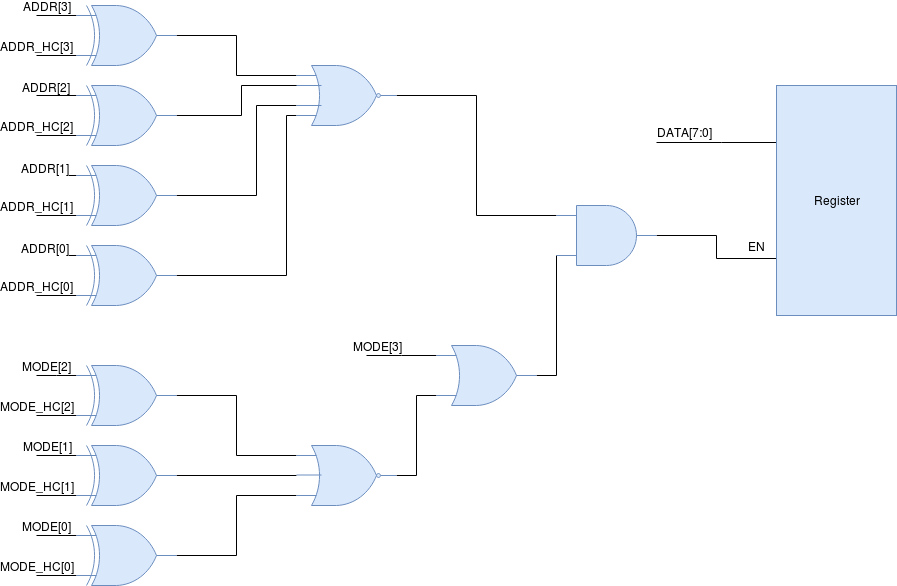
\includegraphics[scale=.45,keepaspectratio=true]{./ch3_figures/Register.png}
 \caption{Register address and mode decoding}
 \label{fig:register}
\end{figure}

\par The \emph{ADDR} and \emph{MODE} bits are compared against a hard coded value using the XOR and NOR gates. The hard coded values will be set to match the address of the channel the register is in, as well as the mode that should select the specific register. The \emph{ADDR} decoder circuit is then ORed with the MSB of \emph{MODE} so that all registers of a given mode can be selected if the global mode bit is set.

\subsection{Power on reset circuit}
\par A power on reset circuit is used to start the PTAT bias current generator circuit. The POR circuit was used from the provided analog cells library with the AMS design kit. When power is applied to the CFD16C, the power on reset (POR) circuit generates a single low active reset pulse. This reset pulse is guaranteed to be at least 2 $\mu sec$ long. The POR signal pulse is used to start the PTAT current reference. This PTAT current reference circuit can converge on a 11.5 $\mu$A or 0 A output current when the CFD16C first receives power, but the 0 A solution is not useful. This long reset pulse guarantees that the PTAT current generator will start correctly and provide an 11.5 $\mu A$ bias current.

\subsection{Signal ground generator}
\par In each of the signal channels the analog input circuitry is all referenced to a separate signal ground. This signal ground, called \emph{AGND}, must be at a potential half way between \emph{AVDD} and \emph{AVSS}. An analog ground generator circuit was provided in an analog cell library from AMS. The signal ground generator circuit can be trimmed to a specific voltage using three trim bits. The signal ground generator has a nominal reference voltage of 1.63 V and can be trimmed by $\pm 250$ mV.

\subsection{Bandgap voltage reference}
\par A bandgap voltage reference is a circuit that provides a temperature and power supply independent voltage \cite{ALLEN}. The bandgap voltage reference used in this design was provided in an analog cells library, and is a known working design. The bandgap voltage reference is used to provide a 1.2 V reference point that is independent of temperature or power supply noise. The bandgap voltage is created by generating a PTAT series resistor and a diode-connected parasitic bipolar PNP transistor \cite{ALLEN}. The PTAT current has a positive temperature coefficient while the PNP transistor has a negative temperature coefficient creating a nodal voltage with a temperature coefficient of only -87 $\frac{\mu V}{^{\circ}C}$ as can be seen in Figure~\ref{fig:bandgap}.
\par This bandgap topology produces an output voltage of $\approx 1.2 V$ with near zero temperature independence. The bandgap reference is further filtered by an RC lowpass filter before being used by any other circuits. This is mostly due to the sensitivity of the circuits that use the bandgap reference to noise, rather than an inherently noisy bandgap reference.

\begin{figure}[htbp!]
\centering
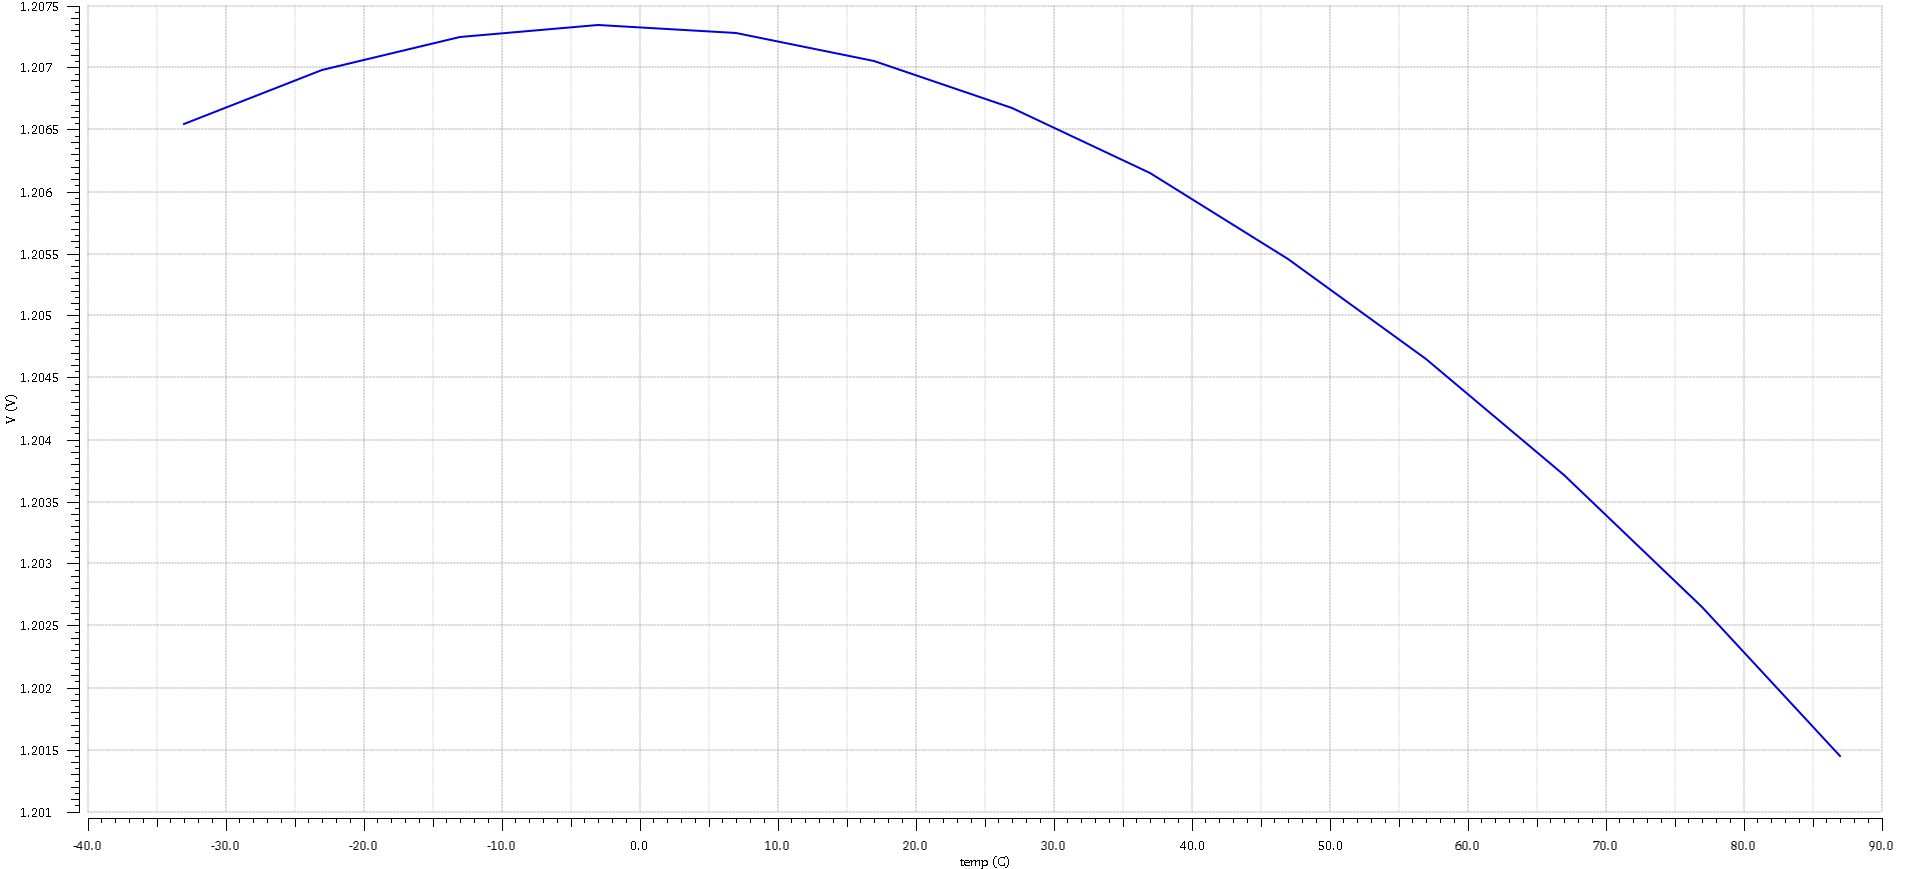
\includegraphics[scale=.3,keepaspectratio=true]{../data/bandgap_temp.png} 
\caption{Bandgap temperature dependence.}
\label{fig:bandgap}
\end{figure}

\subsection{PTAT current reference}
\par A PTAT current reference was used from the analog cells library provided by AMS. This current reference produces a bias current between 7.3 $\mu$A and 17.8 $\mu$A with a nominal value of 11.5 $\mu$A. This bias current is proportional to absolute temperature and is used to bias all of the amplifiers on the chip. A weakly or moderately inverted FET has a tranconductance linearly proportional to bias current but inversely proportional to absolute temperature. Thus by using PTAT currents for the moderately inverted FETs in the amplifier designs, the transconductance of the FETs becomes independent of temperature \cite{ALLEN}. Figure~\ref{fig:ptat} shows the temperature dependence of the PTAT current reference circuit.

\begin{figure}[htbp!]
\centering
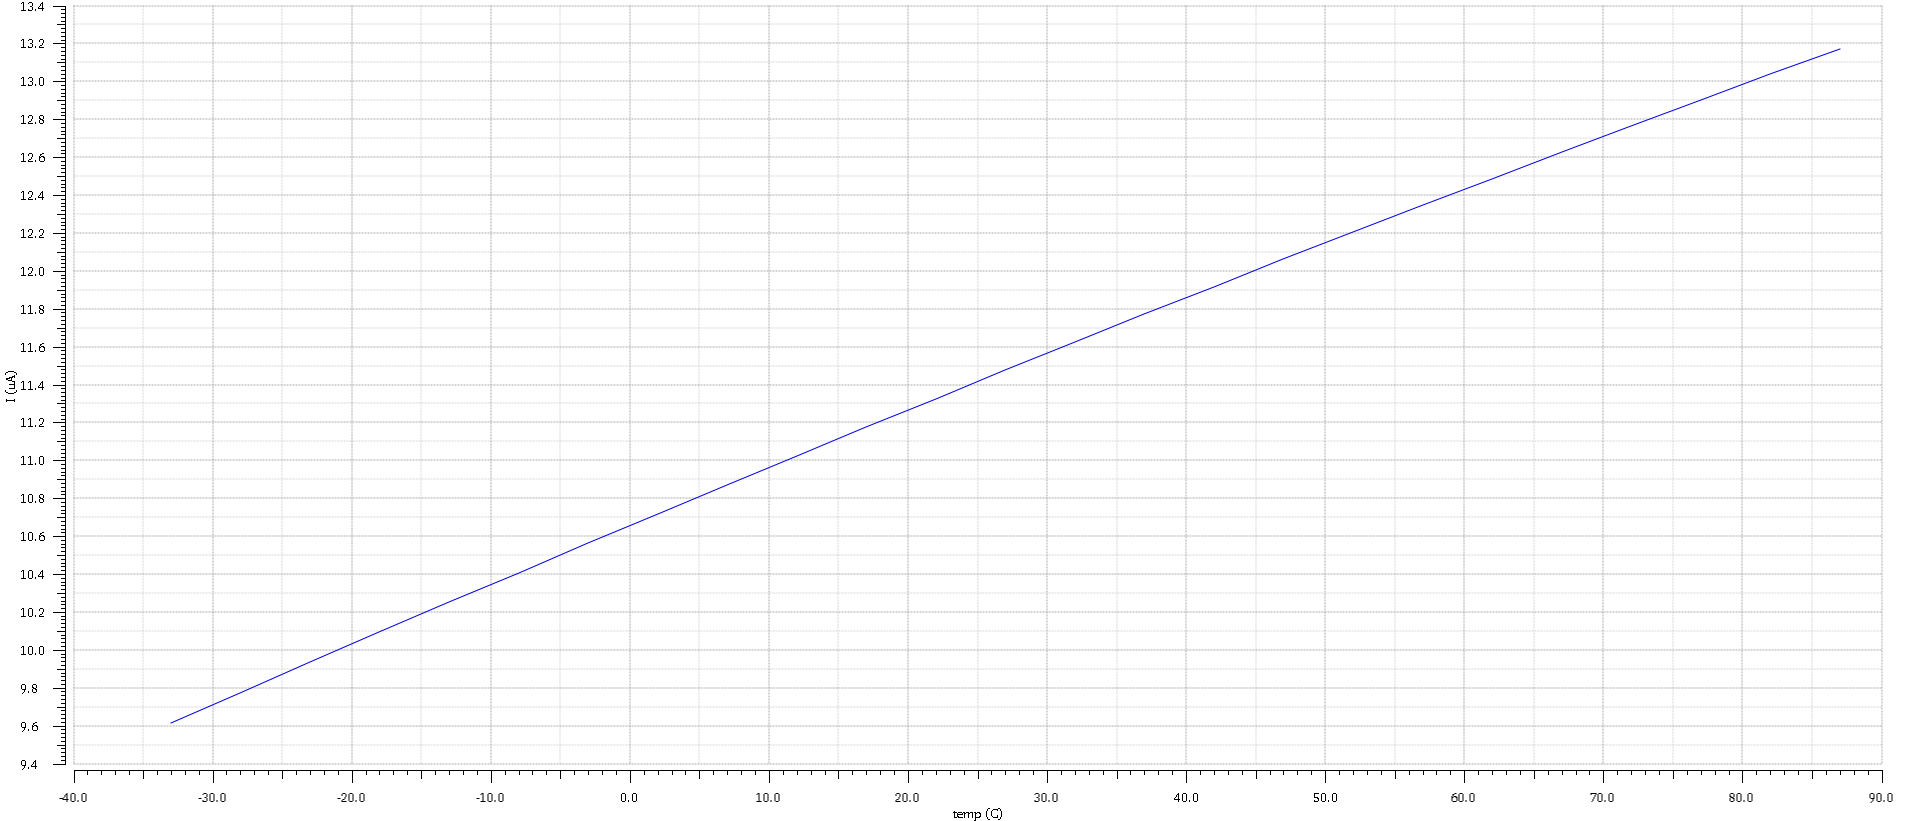
\includegraphics[scale=.3,keepaspectratio=true]{../data/ptat.png} 
\caption{PTAT current reference temperature dependence.}
\label{fig:ptat}
\end{figure}

\subsection{Zero-tempco current reference}
\par In order to function correctly, some of the circuitry in the signal channel needs to be biased with a current that has no temperature dependence. This zero temperature coefficient (ZTC) current was generated using an opamp circuit shown in Figure~\ref{fig:ztc}. In this circuit, the temperature independent bandgap voltage is applied to the inverting terminal of an opamp. The output of the opamp connects to the gate of a PFET whose drain is connected to a zero temperature coefficient 100 k$\Omega$ resistor. A feedback connection to the non-inverting terminal of the opamp is made to the drain of the PFET as well. 
\par Because of this feedback connection, the opamp will drive the gate of the PFET to a voltage that ensures there is no potential difference between the inverting and non-inverting terminals of the opamp. This means the voltage drop across the ZTC resistor has to be equal to the bandgap voltage and so the current through the PFET has to be 12 $\mu$A. This ZTC current reference produces a current with a temperature dependence of only 2.07 $\frac{nA}{^{\circ}C}$ as seen in Figure~\ref{fig:ztc-temp}.
\par The ZTC resistor is made from a resistor with positive temperature coefficient (rpoly2), and one that has a negative temperature coefficient (rpolyh). The ratio to achieve temperature independence in this process is $\approx$0.56 rpoly2 to 0.44 rpolyh. Since a 12 $\mu$A ZTC current is desired, a 100 k$\Omega$ resistor was made using a 56 k$\Omega$ rpoly2 resistor and a 44 k$\Omega$ rpolyh resistor. This ZTC current is replicated using 17 current mirrors to provide one for each channel, as well as one for the lockout DAC in the common channel. The ZTC currents are used to give the DAC circuits an output that doesn't depend on temperature.
\begin{figure}[htbp!]
\centering
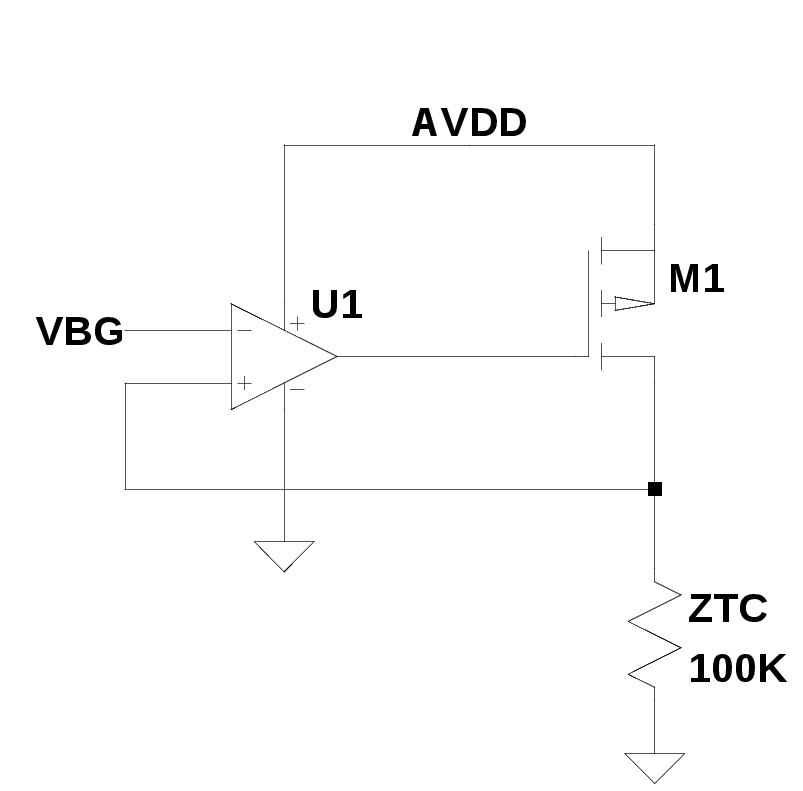
\includegraphics[scale=.36,keepaspectratio=true]{../LTspice_Drawings/ztc_iref/circuit.png} 
\caption{Zero temperature coefficient current generator.}
\label{fig:ztc}
\end{figure}

\begin{figure}[htbp!]
\centering
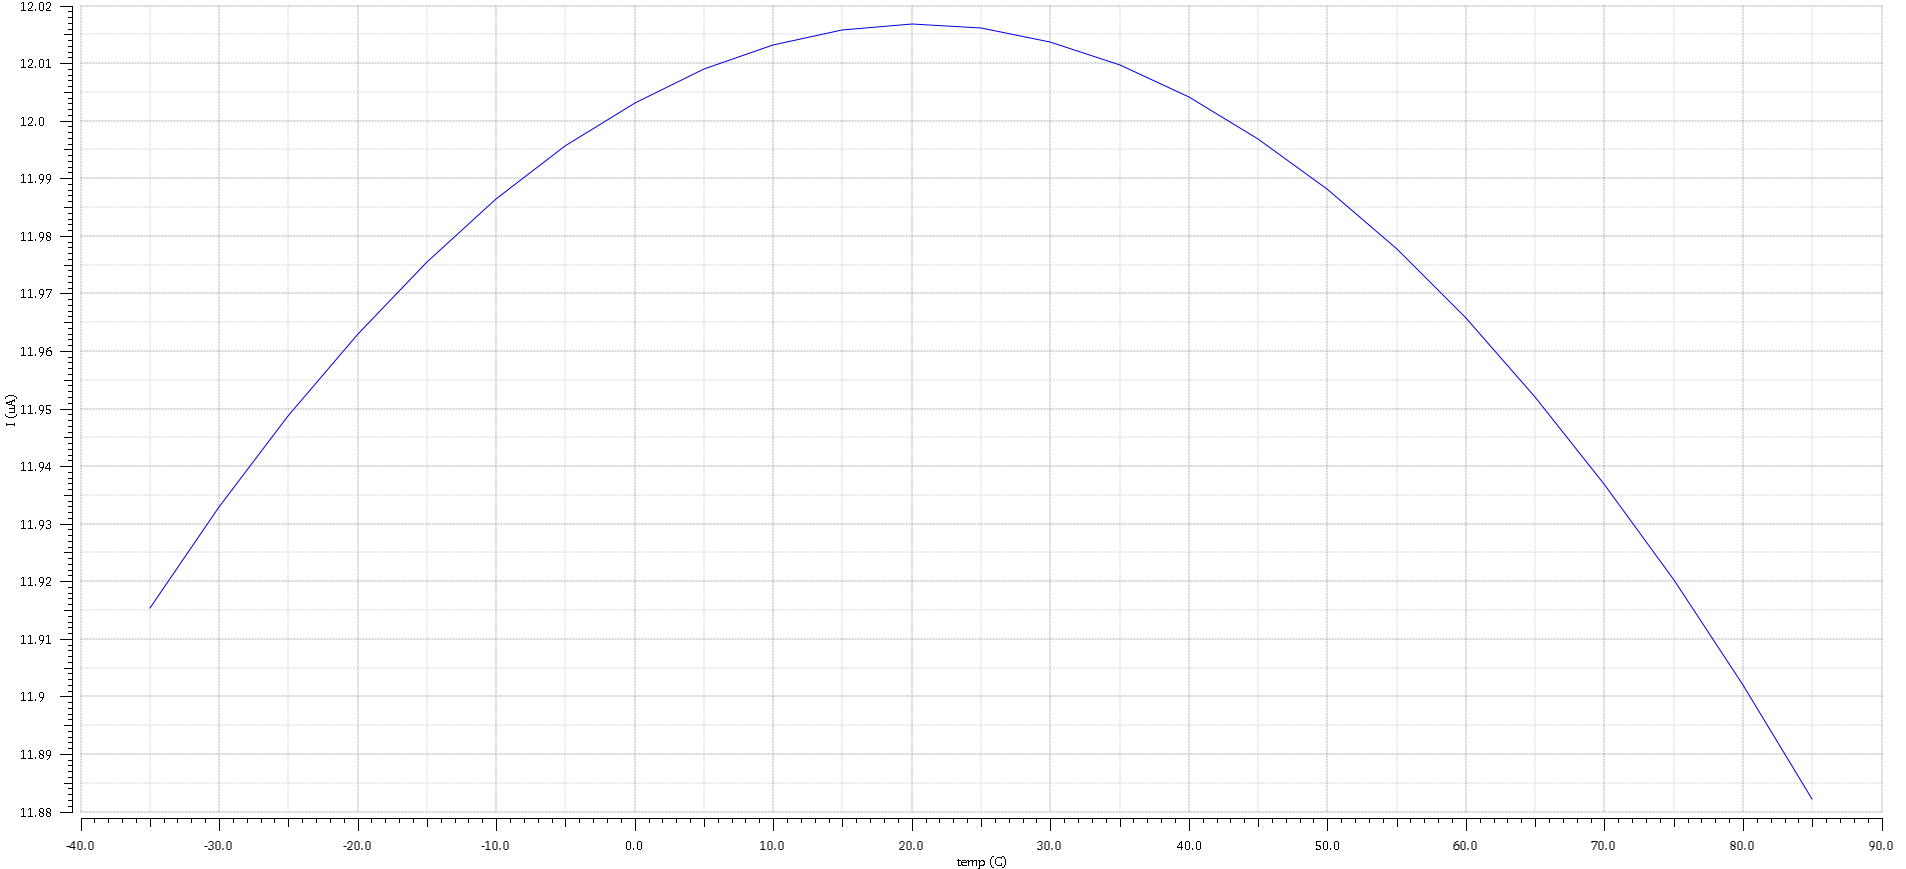
\includegraphics[scale=.3,keepaspectratio=true]{../data/ztc.png} 
\caption{Zero temperature coefficient current temperature dependence.}
\label{fig:ztc-temp}
\end{figure}

\subsection{Lockout DAC}
\par It is desirable to prevent the one-shot circuit in the signal channels from firing for a set amount of time after it has already fired. The length of this lockout time may need to change depending on the nature of the experiment. To do this, a lockout time can be set that is proportional to the voltage at the output of a 6-bit digital to analog converter (DAC). 
\par The DAC itself is implemented as a current scaling DAC using an R2R ladder topology that makes use of MOSFETs as resistors. While MOSFET resistors are generally non-linear and not suitable for use in DAC design, a special technique was used in this design to ensure linearity for current division \cite{DAC}. This technique allowed for the R2R ladder to be made much smaller than using traditional poly resistors, while having very good current division capabilities.
\par The input to the DAC is a ZTC current coming from the common channel. The R2R ladder equally divides the input current in half and uses this divisor current as the input to the next stage of the DAC, as seen in Figure~\ref{fig:dac-block}. The other half of the current is mirrored using a cascode current mirror to create part of the output current of the DAC (Figure~\ref{fig:dac}). The use of a cascode current mirror an extremely high output impedance of $r_{ds7}\cdot g_{m7} \cdot r_{ds6}$. A terminator circuit is used to ensure the current splits in half for the last stage (Stage0).

\begin{figure}[htbp!]
\centering
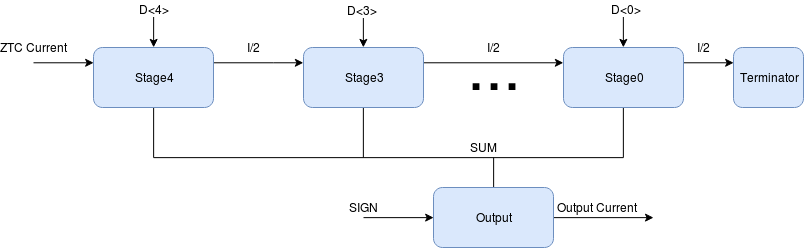
\includegraphics[scale=.55,keepaspectratio=true]{./ch3_figures/dac.png} 
\caption{6-bit bipolar DAC}
\label{fig:dac-block}
\end{figure}

\par The NFET \emph{M8} in Figure~\ref{fig:dac} acts as a switch to only allow current to flow when the control bit, \emph{D<i>}, is a logic 1. The currents are summed up and mirrored with another cascode current mirror in a final output stage of the DAC (Figure~\ref{fig:dac-out}). Either a PFET current mirror or NFET current mirror will be used depending on the sign bit. If the sign bit is high, meaning negative polarity is enabled, then the NFET current mirror will sink current from the DAC output. Conversely, if the sign bit is high, then the PFET current mirror sources current to the output.
\par For the lockout voltage, the DAC will only source current to the output where it is passed through a diode connected NFET to create a voltage. The same DAC design is also used for the leading-edge dsicriminator threshold, and must be bipolar in that design. 

\begin{figure}[htbp!]
\centering

\includegraphics[scale=.4,keepaspectratio=true]{../LTspice_Drawings/dac/dac_stage.png} 
\caption{One stage of DAC using R2R ladder}
\label{fig:dac}
\end{figure}

\begin{figure}[htbp!]
\centering

\includegraphics[scale=.6,keepaspectratio=true]{../LTspice_Drawings/dac/dac_out.png} 
\caption{DAC output current stage}
\label{fig:dac-out}
\end{figure}

\subsection{Multiplicity output buffer}
\par One of the outputs of the CFD16C is an analog voltage that is proportional to the number of channels that have fired. To create this output each of the signal channels outputs a copy of the PTAT current but only when the channel has fired. All of these PTAT currents are summed up using a resistor to create a voltage. However, it is necessary to buffer this output voltage before sending it off chip. For this a source follower output buffer is used to present a high input impedance, but low output impedance of $\frac{1}{g_{m M_{2}}}$. 
\par The source follower circuit, shown in Figure~\ref{fig:mult}, is biased with a 1 mA current using resistor R1. The signal channel multiplicity currents are summed up using R2 creating an output voltage on the source of M3. This output voltage is 1.15 V when no channels have fired and 2.7 V when all sixteen channels have fired. 

\begin{figure}[htbp!]
\centering

\includegraphics[scale=.45,keepaspectratio=true]{../LTspice_Drawings/multiplicity/mult_buffer.png} 
\caption{Multiplicity output buffer.}
\label{fig:mult}
\end{figure}

% DESCRIPTION OF SIGNAL CHANNEL

\section{Signal Channel}
\par The CFD16C is made up of sixteen signal channels capable of producing a precise output pulse. Each of the signal channels is identical but contain configurable analog blocks that can be changed on a per channel basis. The signal channel consists of a Nowlin circuit, leading-edge detector circuit, zero-crossing detector circuit, a one-shot circuit, and an output generation circuit. 

\subsection{Programmable Nowlin circuit}
\par The Nowlin circuit is used at the input stage of each of the signal channels and is shown in Figure~\ref{fig:Nowlin}. The Nowlin circuit turns a single ended input pulse into a differential signal for use in the zero crossing discriminator. This is achieved by taking a fraction, in this case $\frac{2}{3}$, of the input voltage using a resistor voltage divider (ZC-). The other leg (ZC+) of the differential output is a delayed version of the input pulse. The delay comes from resistor R3 in Figure~\ref{fig:Nowlin} and the programmable capacitor C2. This creates a configurable RC time constant to delay the input signal. 
\begin{figure}[ht]
\centering

\includegraphics[scale=.3,keepaspectratio=true]{../LTspice_Drawings/nowlin/nowlin.png} 
\caption{Nowlin circuit.}
\label{fig:Nowlin}
\end{figure}
\par C1 and the series combination of R1 and R2 create a high pass filter whose output is called LE+. The corner frequency of this high pass filter is given by $f_{c} = \frac{1}{2\pi \cdot(\frac{R1 \cdot R2}{R1 + R2})\cdot C2} \approxeq 475  kHz$. This high pass filter output is used as input the the leading edge discriminator. The reason for high pass filtering is to remove any low frequency and DC noise present on the input pin as the actual signal pulse will always be a high frequency exponential pulse.
\par The programmable capacitor (C2) in the Nowlin circuit is created by using switches, in this case transmission gates, to connect individual capacitors in and out of circuit with the Nowlin. Two transmission gates (t-gates) per capacitor are used to accomplish this. The programmable capacitor circuit can be seen in Figure~\ref{fig:pcap}.
\par In this configuration when a bit from the programmable capacitor bus is on (ie. 3.3V), the capacitor connects in parallel with C1 from Figure~\ref{fig:pcap}, adding more capacitance to the ZC+ node in the Nowlin circuit. If the control signal is off (ie. 0V) then the capacitor is shorted out to \emph{AGND} discharging it and removing capacitance from the ZC+ node. In total there are four of these capacitor circuits, one for each bit of the programmable capacitor bus. Each capacitor is binary weighted with the following values: 0.5 pF, 1 pF, 2 pF, and 4 pF. This gives a total in circuit capacitance of 8 pF and a minimum in circuit capacitance of 0.5 pF. Table~\ref{tab:pcap} shows the bit order of these capacitor elements. Referencing this table shows that the total capacitance at the ZC+ node will be $C_{total} = D \cdot 0.5 pF + 0.5 pF$ where D is the decimal value of the 4-bit programmable capacitor bus.
\par The programmable capacitor must be set properly in order to ensure proper operation of the signal channel. Using Table~\ref{tab:pcap} an appropriate time constant must be set. This time constant should be chosen such that it is as close as possible to the rise time constant expected from the exponential input pulses coming into the Nowlin circuit.
\begin{figure}[htbp!]
\centering

\includegraphics[scale=.4,keepaspectratio=true]{../LTspice_Drawings/nowlin/pcap.png} 
\caption{Programmable capacitor circuit.}
\label{fig:pcap}
\end{figure}
\begin{table}[htbp!]
 \centering
 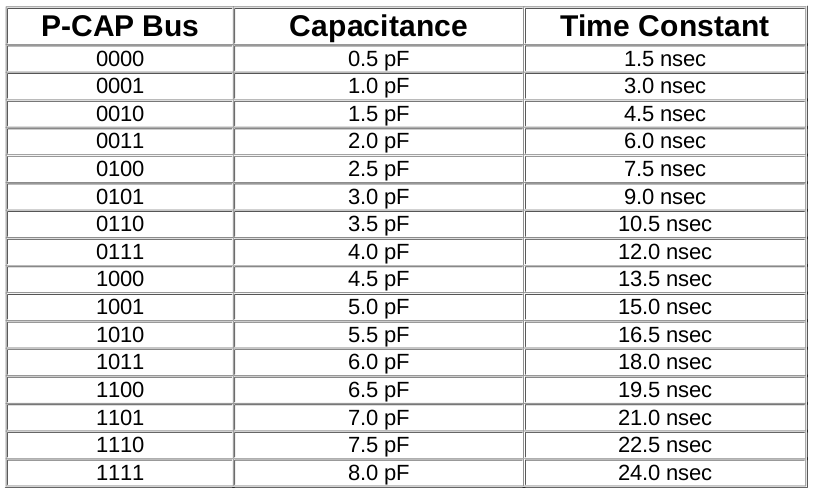
\includegraphics[scale=.35,keepaspectratio=true]{../data/pcap.png}
 \caption{Programmable capacitor values and time constants.}
 \label{tab:pcap}
\end{table}

\subsection{Leading-edge discriminator}

\subsection{Zero-cross discriminator}


\subsection{Output one-shot with lockout features}
\par The output timing pulse for each of the channels is generated from a one-shot circuit with lockout capabilities. A one-shot circuit is a circuit that creates a fixed width output pulse in response to a narrow input pulse. The one-shot circuit in the signal channels is what produces the output timing pulse used to start the TVCs on the PSD8C. The one-shot circuit design is shown in Figure~\ref{fig:oneshot-circuit}.

\begin{figure}[htbp!]
\centering
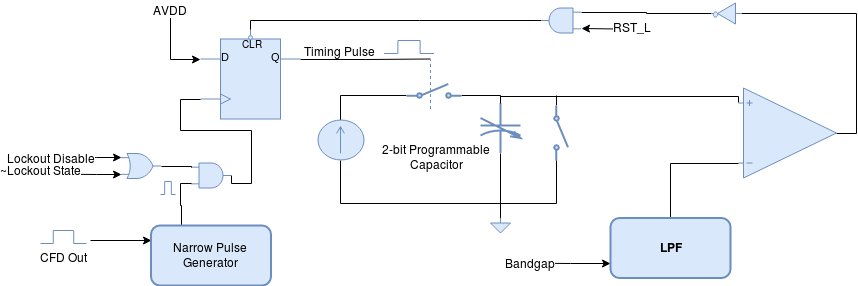
\includegraphics[scale=.50,keepaspectratio=true]{./ch3_figures/oneshot_circuit.png} 
\caption{One-shot circuit with lockout}
\label{fig:oneshot-circuit}
\end{figure}

\par The one-shot circuit works but utilizing a D-type flip flop with an asynchronous clear input. When the CFD circuit (ie. Leading-edge and Zero-cross discriminators) produces an output, the pulse width can be variable depending on the conditions in the experiment. Because of this a narrow pulse generator is used to produce a fixed 5 nsec wide pulse in response to any width CFD output. This narrow pulse is used as a clock signal for this D-flip flop, provided lockout is disabled or the circuit is not in a lockout state. Since the input to the flip flop is tied to \emph{AVDD} (logic high) the output will transition to a logic high state in response to the CFD circuit output. This causes a switch to close allowing a current source to charge a capacitor at the input of a comparator. Charging this capacitor produces a ramp voltage on the non-inverting input of the comparator, as seen in Figure~\ref{fig:ramp}.

\begin{figure}[htbp!]
\centering
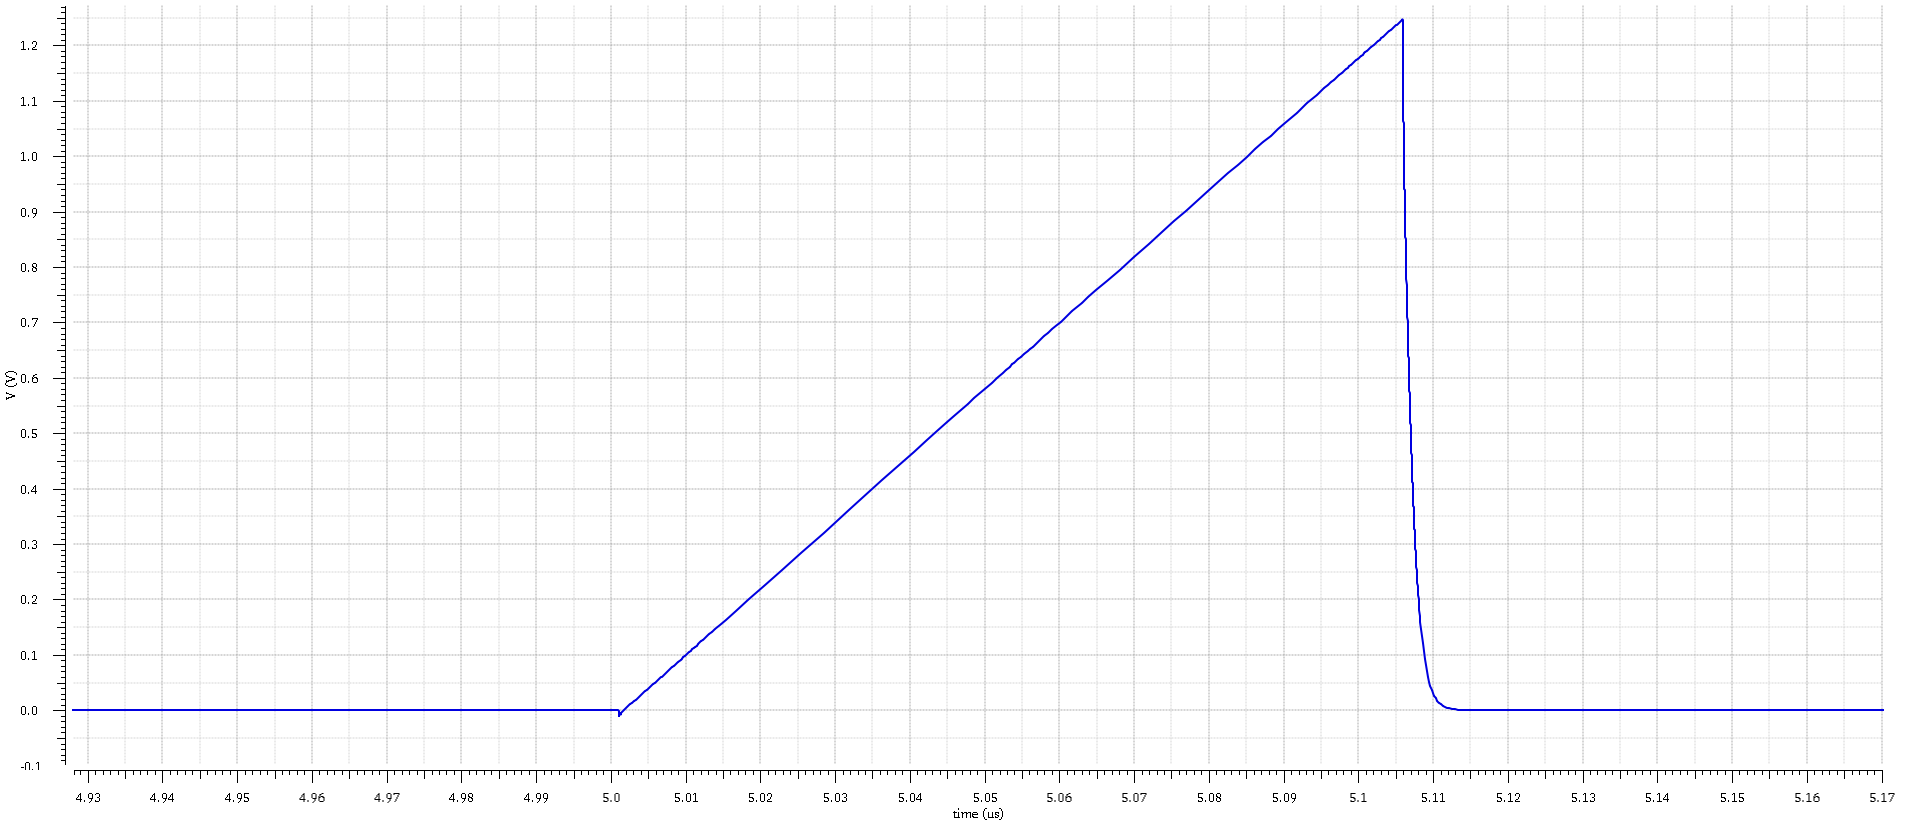
\includegraphics[scale=.3,keepaspectratio=true]{./ch3_figures/ramp.png} 
\caption{Comparator ramp input}
\label{fig:ramp}
\end{figure}

\par The inverting input to the comparator is connected to a low pass filtered bandgap voltage. Thus, when the ramp input reaches 1.2 V the comparator output a logic high. The comparator output triggers the \emph{CLR} input on the D-flip flop to go low, forcing the output of the flip flop into a logic low state. This causes the switch controlling the current source to open and the switch in parallel with the capacitor to close, shorting the capacitor out and discharging it. The \emph{CLR} input on the flip flop can also be triggered by a master reset provided by the \emph{RST\_L} pin on the CFD16C. 

\par By changing the value of the programmable capacitor the charge time changes, effectively changing how long the D-flip flop will be in the logic high state (ie. it sets the width of the timing pulse). The lockout one-shot circuit works on a similar principle but has a non-programmable capacitor (250 fF) with a programmable charge current. Changing the charge current allows the capacitor to charge faster or slower, changing the lockout time. Two lockout modes are also available by writing to a mode bit as seen in Table~\ref{tab:modes}. When Lockout Mode is a logic high, shorter $\approx$110 nsec time incremented are provided for a total lockout time of 3.4 $\mu$sec. When the Lockout Mode is a logic low, a long mode is used providing $\approx$565 nsec increments for a total lockout time of 16.6 $\mu$sec. The lockout one-shot provides an active low output as opposed to the active high output of the timing pulse one-shot.

\subsection{Final output generation}
\par All of the signal channel output are generated in a final output generation stage. In this stage the timing pulse, multiplicity current, global OR, and test point outputs are produced. While the timing pulse is generated in the previous stage by the one-shot circuit, it is necessary to further qualify this output before sending it off chip. Each signal channel can be individually enabled or disabled using a configuration bit, or the whole CFD16C chip can be disabled using a global enable input pin. If the global enable signal or the channel enable bit are not asserted then the timing pulse from the one shot will not be present on the output pin and will not trigger the global OR output. 
\par A number of test point nodes from within the channel can be selected to be routed to a pin on the chip package. These available test point nodes are detailed in Table~\ref{tab:test-point}. A multiplexer at the end of each channel controls which test point is used. To prevent all sixteen channels from trying to drive the test point pin at once, a tri-state buffer with enable is used. This enable signal will only be active for the channel whose address is currently selected on the \emph{ADDR} bus, and all other channels will have their test point outputs put into a high impedance state.  

\begin{table}[ht]
 \centering
 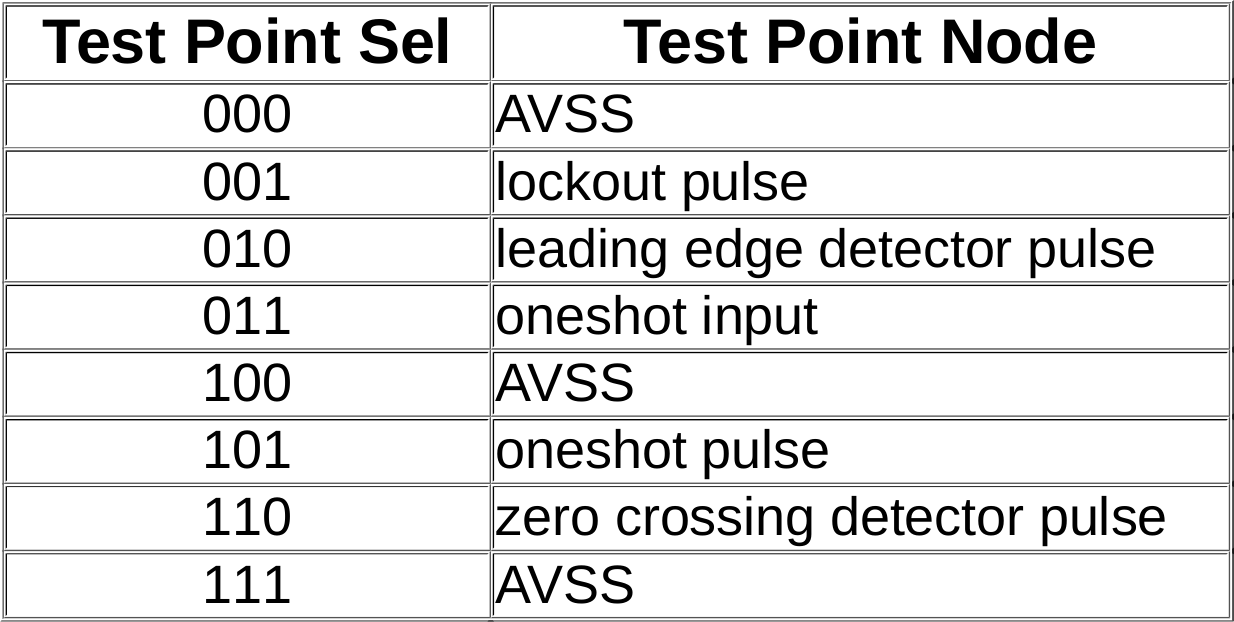
\includegraphics[scale=.2,keepaspectratio=true]{../data/test_points.png}
 \caption{Test point multiplexer outputs}
 \label{tab:test-point}
\end{table}

\par The multiplicity current is produced in response to the timing pulse output firing. Once the timing pulse has fired and been qualified, a PFET switch is turned on and allows a copy of the PTAT current to be sourced to the multiplicity buffer in the common channel. All of the channel multiplicity current output are sourced to the same node so that the voltage across the resistor in the multiplicity buffer will be determined by the sum of all of the currents from the fired channels. 
\par The global OR signal is produced by the timing pulse as well. This output is generated using a pseudo-NMOS NOR gate. As shown in Figure~\ref{fig:pseudo-nmos}, in a pseudo-NMOS NOR gate a PFET acts as a pullup for parallel connected NFETs \cite{WESTE}. Thus if any one NFET is turned on then the output node will be pulled to \emph{AVSS}. Each channel contains one of these NFETs with the PFET and a CMOS inverter being in the common channel. This allows for a very fast active high logic OR of all of the channels with reduced complexity since the NOR gate is distributed across all channels (reducing the amount of interconnect needed).

\begin{figure}[htbp!]
 \centering
 
\includegraphics[scale=.35,keepaspectratio=true]{../LTspice_Drawings/pseudo-nmos/pseudo-nmos.png}
 \caption{Fast pseudo-NMOS NOR}
 \label{fig:pseudo-nmos}
\end{figure}

% ^^^^^^^^^^^^^^^^^^^^^^^^^^^^^^^^^^^^^^^^^^^^^^^^^^^^^^^^^
%  CHAPTER 4
% ^^^^^^^^^^^^^^^^^^^^^^^^^^^^^^^^^^^^^^^^^^^^^^^^^^^^^^^^^


\chapter{SIMULATION RESULTS}

\section{Verification of Circuits in Common Channel}

\section{Walk Characteristics of CFD Circuit}

\section{Jitter Performance}

\section{Verification of One-Shot}

\par The output one-shot provides two important features to the CFD16C: generation of the timing pulse that starts the TVCs on PSD8C, and a lockout functionality to prevent misfirings. For the lockout feature a wide spread of lockout times was desired, with a logarithmic spread. Figure~\ref{fig:lockout-spread} shows the spread of the lockout times available in both the short and long modes. As can be seen from the plots the spread is nearly logarithmic, with the lockout time being given by $T_{lockout} = \frac{K}{D\cdot \Delta I}$, where K is determined by $K = C\cdot V_{C}$ (C is capacitor in lockout one-shot), D is the digital code word given to the lockout DAC, and $\Delta$I is the change in current from one step of the lockout DAC. The $\Delta$I term will change depending on the lockout mode, being 380 nA in short mode and 3.8 nA in long mode. 

\begin{figure}[htbp!]
 \centering
 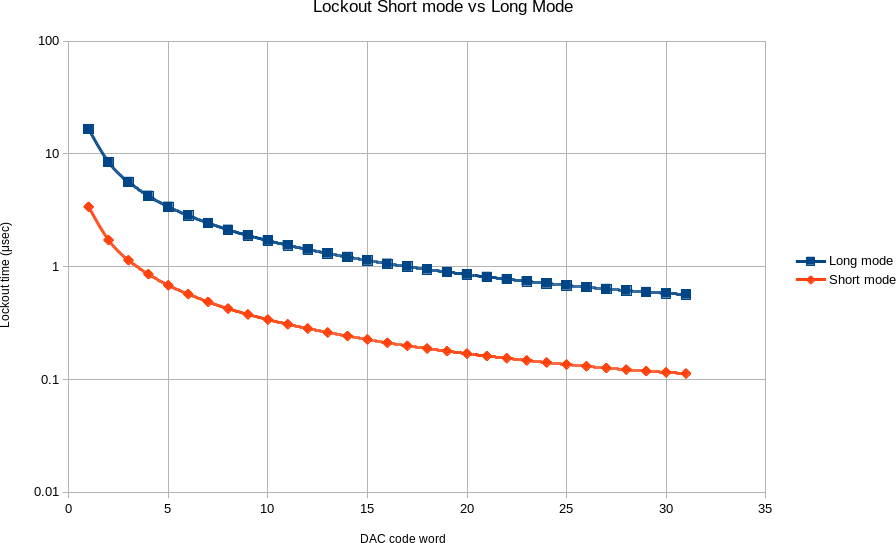
\includegraphics[scale=.63,keepaspectratio=true]{./ch4_figures/lockout_plot.png}
 \caption{Lockout times for short and long modes}
 \label{fig:lockout-spread}
\end{figure}

\par The primary one-shot that creates the output timing pulse needs very low jitter and low variance from process and mismatch. The jitter proved to be accurately modeled by the formula $\sigma_{j} = \frac{\sigma_{V}}{V{BG}}\cdot T_{oneshot}$, where $\sigma_{V}$ is the noise voltage in the current source (PFET current mirror) charging the one-shot capacitor in Figure~\ref{fig:oneshot-circuit} and V$_{BG}$ is the bandgap voltage. For process variance and mismatch, 20 Monte Carlo simulations were run and showed acceptable variance in the trailing edge of the one-shot timing pulse (Table~\ref{tab:one-shot-mc}). This result is within two sigma, and it is expected that across all process and mismatch a variance of no more than $\pm$5 nsec in the trailing edge of the one-shot pulse is expected.

\begin{table}[htbp!]
 \centering
 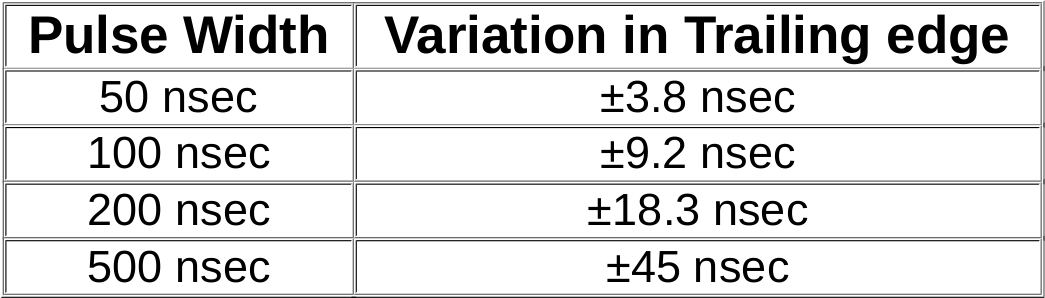
\includegraphics[scale=.25,keepaspectratio=true]{../data/oneshot_mc.png}
 \caption{One-shot pulse width variation from process and mismatch}
 \label{tab:one-shot-mc}
\end{table}

\section{Performance Characterization of DAC}
\par The 6-bit bipolar DAC needed to have excellent integral non-linearity error (INL) and derivative non-linearity error (DNL) of less than 0.5 least significant bits (LSBs). Derivative non-linearity describes how much the output changes for each increment of the digital code word for the DAC \cite{ALLEN}. In an ideal DAC this change would be exactly the same for each increment but in reality there are minor differences between each increment. The accumulation of all of these DNL errors over the whole range of the DAC is the INL error \cite{ALLEN}. 

\par Figures~\ref{fig:dnl}--\ref{fig:inl} show the results of 200 Monte Carlo simulations. With each separate Monte Carlo simulation, the values of the process parameters such offset voltages, threshold voltages, etc. will be assigned differently allowing for process variation from chip to chip to be examined. As can be seen the INL and DNL errors are almost all below 0.5 LSBs with only a few outliers. It can also be seen that the worst case INL and DNL occured on simulation 150.

\begin{figure}[htbp!]
 \centering
 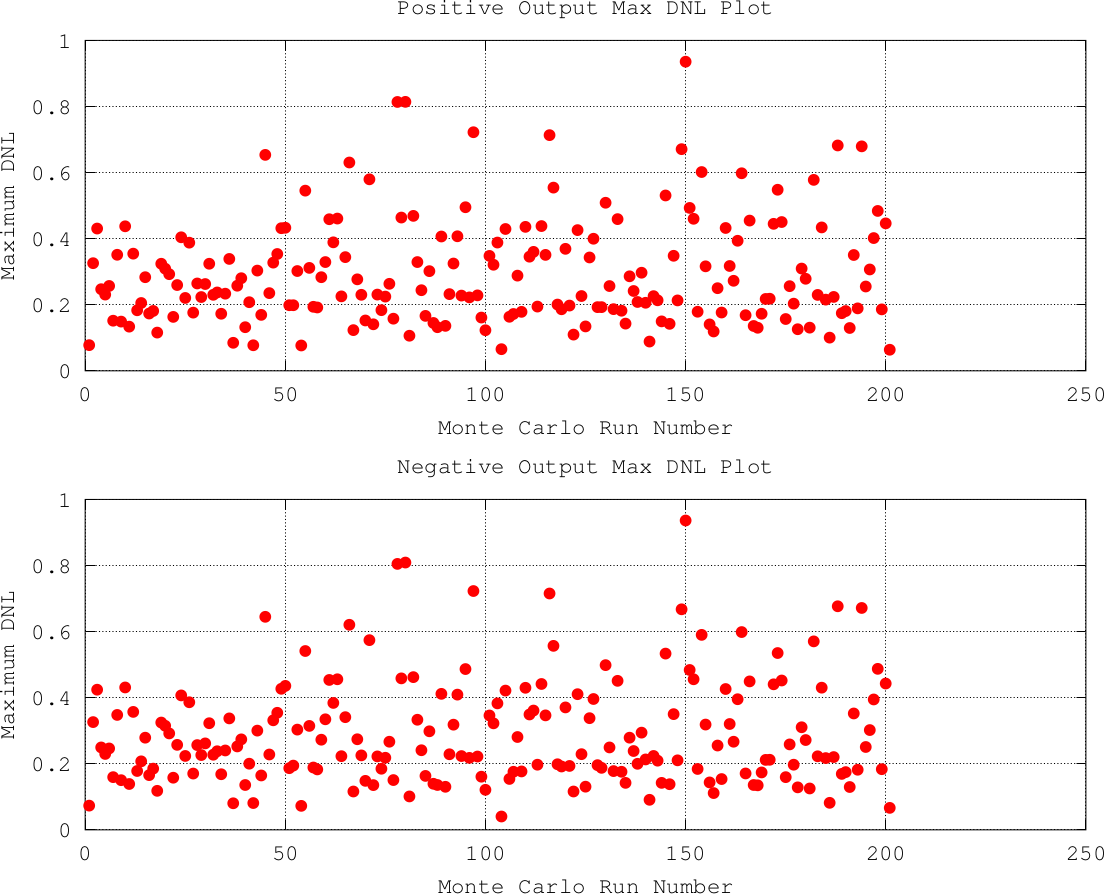
\includegraphics[scale=.31]{./ch4_figures/dnl_summary.png}
 \caption{6-bit DAC DNL error summary}
 \label{fig:dnl}
\end{figure} 

\begin{figure}[htbp!]
 \centering
 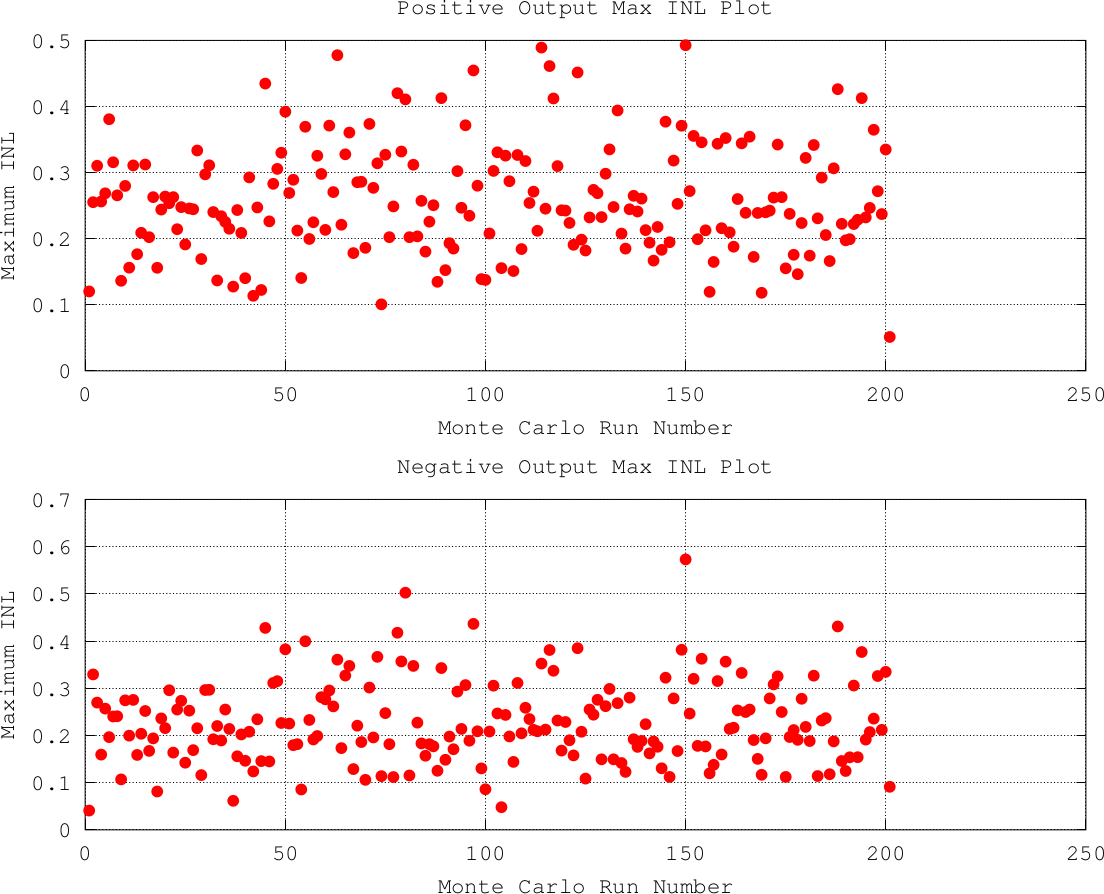
\includegraphics[scale=.31]{./ch4_figures/inl_summary.png}
 \caption{6-bit DAC INL error summary}
 \label{fig:inl}
\end{figure} 

\par Figure~\ref{fig:dac-worst} shows the worst case run out of all 200 simulations. It can easily be seen here than the DNL is well below 0.5 LSB for all increments of the code word except at the half way point. Examining other simulation plots show that this is the case for the other outliers as well, showing that the INL and DNL errors are in general very good and more than acceptable for this application. An average case simulation result is shown below in Figure~\ref{fig:dac-average}, showing that on average the INL and DNL errors are very good.

\begin{figure}[htbp!]
 \centering
 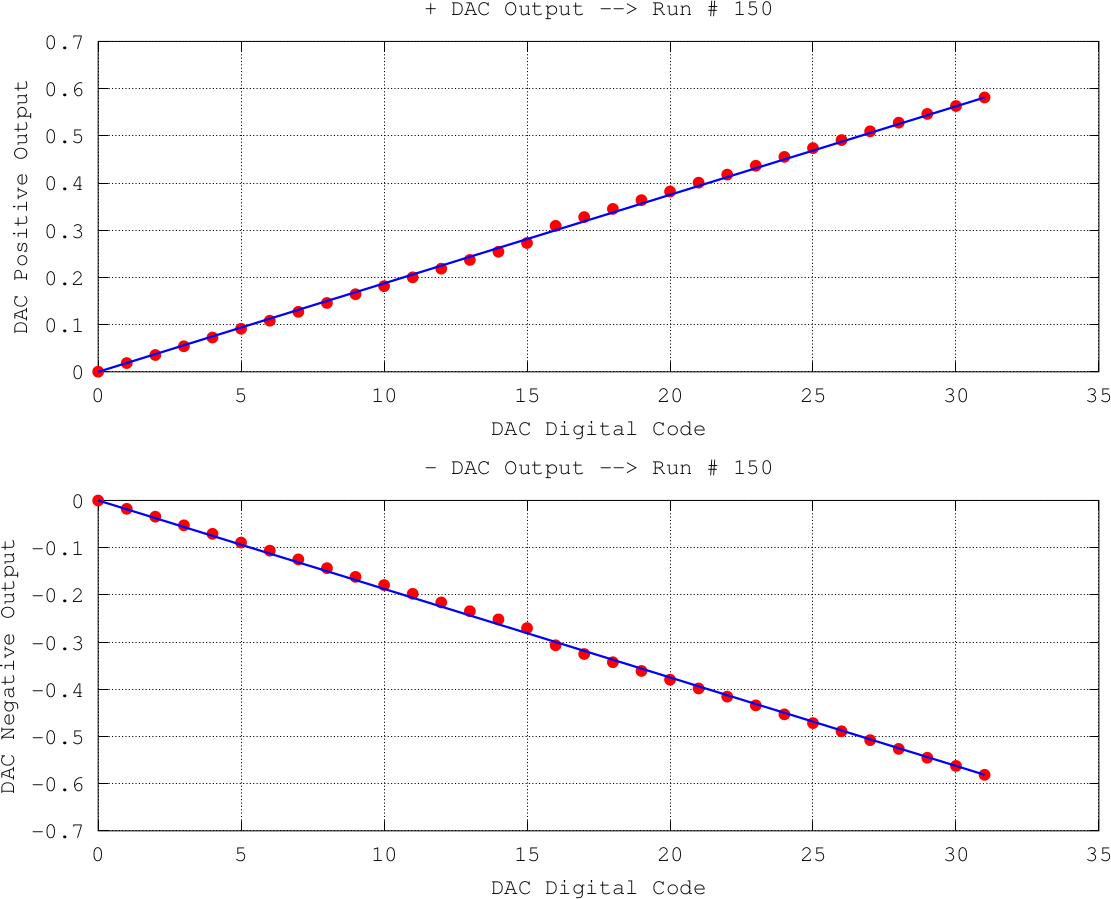
\includegraphics[scale=.31]{./ch4_figures/dnl_worst.png}
 \caption{6-bit DAC worst case error}
 \label{fig:dac-worst}
\end{figure} 

\begin{figure}[htbp!]
 \centering
 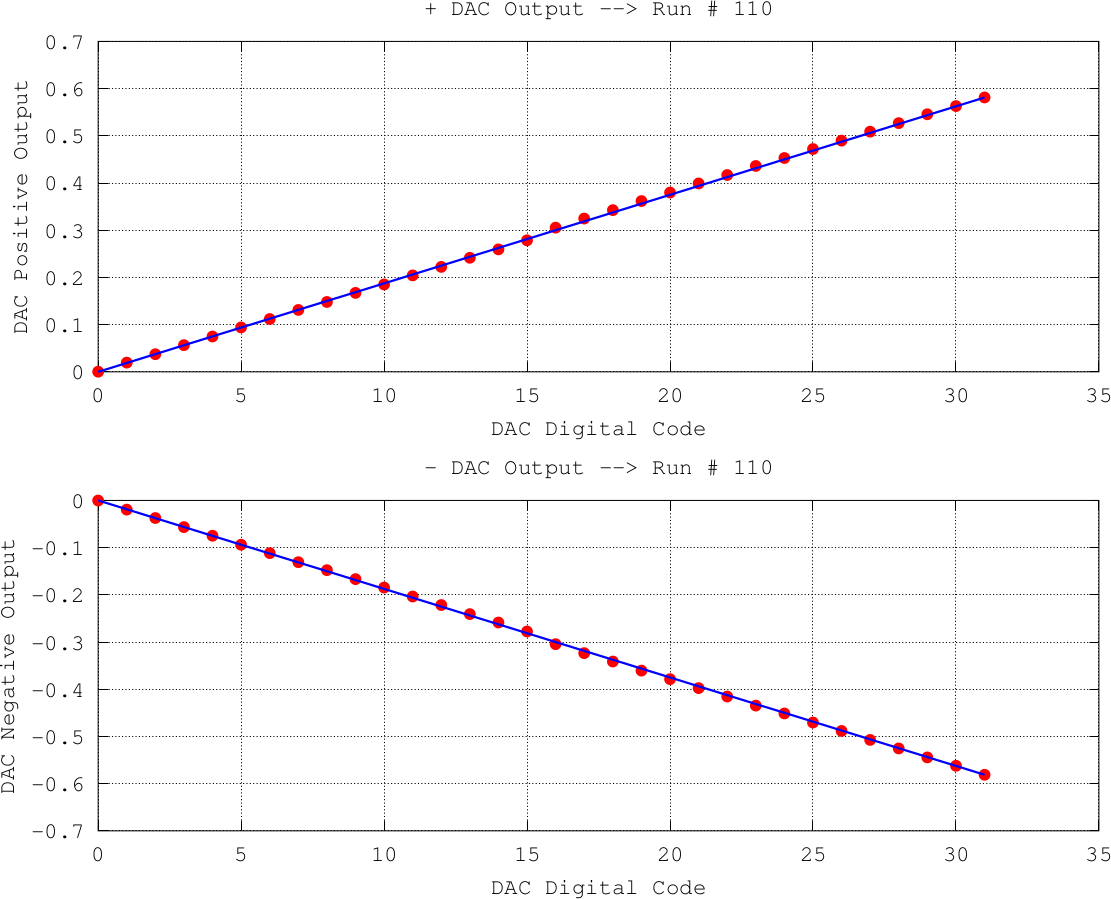
\includegraphics[scale=.31]{./ch4_figures/dac_average.png}
 \caption{6-bit DAC average case error}
 \label{fig:dac-average}
\end{figure} 

\section{Chip-Level Verification}


% ^^^^^^^^^^^^^^^^^^^^^^^^^^^^^^^^^^^^^^^^^^^^^^^^^^^^^^^^^
%  CHAPTER 5
% ^^^^^^^^^^^^^^^^^^^^^^^^^^^^^^^^^^^^^^^^^^^^^^^^^^^^^^^^^


\chapter{SUMMARY, CONCLUSIONS, AND FUTURE WORK}

\section{Summary}
\par The CFD16C was designed as a companion chip for the pulse shape discriminating IC called PSD8C. CFD16C will allow new experiments to be done with PSD8C that were previously not possible. The chip is highly configurable to allow it to be tailored to the needs of the experiment. 
\par The CFD16C provides a precise timing pulse to start time-to-voltage converters on the PSD8C. 

\section{Conclusions}
\par The chip level simulations show that the CFD16C will work very well in new scintillator experiments accompanied with the PSD8C. The design of the IC is complete and layouts will be finished in time for a late 2018 submission.

\section{Future Work}
\par While the bulk of the design for CFD16C has been completed and the simulated performance looks promising, more robust and detailed simulations still need to be ran before the chip is ready to be sent out for fabrication. It is expected the chip will be sent for fabrication in November 2018. Once the chip has been fabricated a performance analysis on the physical IC will be done and any discrepancies from the simulated performance will be identified. More simulations will then be run to find the cause of these discrepancies. 

\nocite{*}


\references %single spacing / arabic numeral paginations, adds "REFERENCES" to table of contents

%%%% for bibtex

%If you want to use bibtex  use the following lines, where your .bib file is called 'yourbib.bib'

\bibliographystyle{apalike}
\bibliography{./Orabutt_Thesis}

% If you have only a single appendix, do it this way.

\multipleappendices
\lstset{
         language=C,
         basicstyle=\scriptsize\ttfamily,
         emptylines=0, 
         lineskip=1pt,
         %numbers=left,            
         numberstyle=\tiny,         
         stepnumber=2,              
         numbersep=5pt,             
         tabsize=3,                
         extendedchars=true,       
         breaklines=true,            
         commentstyle=\color{blue},
         keywordstyle=\color{red},
            frame=b,         
 %        keywordstyle=[1]\textbf,    
 %        keywordstyle=[2]\textbf,    
 %        keywordstyle=[3]\textbf,  
 %        keywordstyle=[4]\textbf,   \
         stringstyle=\scriptsize\color{green}\ttfamily, 
         showspaces=false,         
         showtabs=false,            
%         xleftmargin=17pt,
%         framexleftmargin=17pt,
%         framexrightmargin=5pt,
%         framexbottommargin=4pt,
         %backgroundcolor=\color{lightgray},
         showstringspaces=false           
 }


\end{document}
